% hier werden alle einstellungen und pakete geladen
% Festlegung des Allgemeinen Dokumentenformats
\documentclass[a4paper,12pt,headsepline]{scrartcl}

% Umlaute unter UTF8 nutzen
\usepackage[utf8]{inputenc}

% Variablen
%Variablen welche innerhalb der gesamten Arbeit zur Verfügung stehen sollen
\newcommand{\titleDocument}{Agile Softwareentwicklung für automobile Anwendungen}
\newcommand{\subjectDocument}{OnePager zum Vortrag\\im Fach Prozessgestaltung in der
Produktentstehung}




% weitere Pakete
% Grafiken aus PNG Dateien einbinden
\usepackage{graphicx}

% Deutsche Sonderzeichen und Silbentrennung nutzen
\usepackage[ngerman]{babel}

% Eurozeichen einbinden
\usepackage[right]{eurosym}

% Zeichenencoding
\usepackage[T1]{fontenc}

\usepackage{lmodern}

\usepackage{siunitx}

% floatende Bilder ermöglichen
%\usepackage{floatflt}

% mehrseitige Tabellen ermöglichen
\usepackage{longtable}

% Unterstützung für Schriftarten
%\newcommand{\changefont}[3]{ 
%\fontfamily{#1} \fontseries{#2} \fontshape{#3} \selectfont}

% Packet für Seitenrandabständex und Einstellung für Seitenränder
\usepackage{geometry}
\geometry{left=2.5cm, right=2.5cm, top=2.5cm, bottom=2.5cm}

% Paket für Boxen im Text
\usepackage{fancybox}

% bricht lange URLs "schön" um
\usepackage[hyphens,obeyspaces,spaces]{url}

% Paket für Textfarben
\usepackage{color}

% Schriftart Helvetica verwenden
\usepackage{helvet}
\renewcommand\familydefault{\sfdefault}

% Mathematische Symbole importieren
\usepackage{amssymb}

%Mathematische Umgebung
\usepackage{amsmath}

%\numberwithin{equation}{chapter}

% auf jeder Seite eine Überschrift (alt, zentriert)
%\pagestyle{headings}

% erzeugt Inhaltsverzeichnis mit Querverweisen zu den Abschnitten (PDF Version)
\usepackage[bookmarksnumbered,pdftitle={\titleDocument},hyperfootnotes=false,pdfborder={0 0 0}]{hyperref}
%\hypersetup{colorlinks, citecolor=red, linkcolor=blue, urlcolor=black}
%\hypersetup{colorlinks, citecolor=black, linkcolor= black, urlcolor=black}

% neue Kopfzeilen mit fancypaket
\usepackage{fancyhdr} %Paket laden
\pagestyle{fancy} %eigener Seitenstil
\fancyhf{} %alle Kopf- und Fußzeilenfelder bereinigen
\fancyhead[L]{\footnotesize{Sarah-Anne Teuner, Rico Steinke\\Master Automotive Systems Engineering}} %Kopfzeile links
\fancyhead[C]{} %zentrierte Kopfzeile
\fancyhead[R]{\footnotesize{Hochschule Heilbronn\\Prozessgestaltung in der Produktentstehung}} %Kopfzeile rechts
\renewcommand{\headrulewidth}{0.4pt} %obere Trennlinie

\fancyfoot[L]{\footnotesize{WS 2022/2023}} %Fußzeile links
\fancyfoot[C]{\thepage} %zentrierte Fußzeile
\fancyfoot[R]{\footnotesize{}} %Fußzeile rechts
\renewcommand{\footrulewidth}{0.4pt} %untere Trennlinie

% für Tabellen
\usepackage{array}

% Runde Klammern für Zitate
%\usepackage[numbers,round]{natbib}

% Schaltet den zusätzlichen Zwischenraum ab, den LaTeX normalerweise nach einem Satzzeichen einfügt.
%\frenchspacing

% Paket für Zeilenabstand
\usepackage{setspace}

% für Bildbezeichner
\usepackage{capt-of}

% für Stichwortverzeichnis
\usepackage{makeidx}

% für Listings
\usepackage{listings}
\lstset{numbers=left, numberstyle=\tiny, numbersep=5pt, keywordstyle=\color{blue}\bfseries, stringstyle=\ttfamily,showstringspaces=false,basicstyle=\footnotesize,captionpos=b,commentstyle=\color{green},}
\lstset{language=java}

\lstdefinelanguage{JavaScript}{
	keywords={typeof, new, true, false, catch, function, return, null, catch, switch, var, if, in, while, do, else, case, break},
	keywordstyle=\color{blue}\bfseries,
	ndkeywords={class, export, boolean, throw, implements, import, this},
	ndkeywordstyle=\color{darkgray}\bfseries,
	identifierstyle=\color{black},
	sensitive=false,
	comment=[l]{//},
	morecomment=[s]{/*}{*/},
	commentstyle=\color{purple}\ttfamily,
	stringstyle=\color{red}\ttfamily,
	morestring=[b]',
	morestring=[b]"
}

% Indexerstellung
\makeindex

% Abkürzungsverzeichnis
\usepackage[german]{nomencl}
\let\abbrev\nomenclature

% Abkürzungsverzeichnis LiveTex Version
% Titel des Abkürzungsverzeichnisses
\renewcommand{\nomname}{Abkürzungsverzeichnis}
% Abstand zwischen Abkürzung und Erläuterung
\setlength{\nomlabelwidth}{.25\textwidth}
% Zwischenraum zwischen Abkürzung und Erläuterung mit Punkten
\renewcommand{\nomlabel}[1]{#1 \dotfill}
% Variation des Abstandes der einzelnen Abkürzungen zu einander
\setlength{\nomitemsep}{-\parsep}
% Index mit Abkürzungen erzeugen
\makenomenclature
%\makeglossary
\setlength{\parindent}{0em}
% Abkürzungsverzeichnis TeTEX Version
% \usepackage[german]{nomencl}
% \makenomenclature
% %\makeglossary
% \renewcommand{\nomname}{Abkürzungsverzeichnis}
% \AtBeginDocument{\setlength{\nomlabelwidth}{.25\columnwidth}}
% \renewcommand{\nomlabel}[1]{#1 \dotfill}
% \setlength{\nomitemsep}{-\parsep}

% Optional: Einzelne Zeilen am Anfang einer Seite unterdrücken (Schusterjungen)
% \clubpenalty = 10000
% Optional: Einzelne Zeilen am Ende einer Seite unterdrücken (Hurenkinder)
% \widowpenalty = 10000
% \displaywidowpenalty = 10000

\usepackage{tabularx}
\usepackage{multirow}
\usepackage{multicol}
\usepackage{acronym}
\definecolor{red}{rgb}{1,0,0}

% start des dokuments
\begin{document}

% hier werden die Trennvorschläge inkludiert
%hier müssen alle Wörter rein, welche Latex von sich auch nicht korrekt trennt bzw. bei denen man die genaue Trennung vorgeben möchte
\hyphenation{
Film-pro-du-zen-ten
Lux-em-burg
Soft-ware-bau-steins
zeit-in-ten-siv
}


% Titelseite %
\thispagestyle{empty}

\begin{titlepage}


\begin{figure}[t]
 \centering
 %\includegraphics[width=0.6\textwidth]{img/Logo_HHN}
 %Fakultät für Mechanik und Elektronik
 \hspace{7cm}
~~~~~~~~~~
 
\includegraphics[width=0.35\textwidth]{img/HHN_Logo.jpg}
\end{figure}


\begin{verbatim}


\end{verbatim}

\begin{center}
\Large{Hochschule Heilbronn}\\
%\Large{- Campus <Name> -}\\
\end{center}


\begin{center}
\Large{Fakultät für Mechanik und Elektronik}
\end{center}
\begin{verbatim}




\end{verbatim}
\begin{center}
\doublespacing
\textbf{\LARGE{\titleDocument}}\\
\singlespacing
\begin{verbatim}

\end{verbatim}
\textbf{\subjectDocument}
\end{center}
\begin{verbatim}

\end{verbatim}
\begin{center}

\end{center}
\begin{verbatim}

\end{verbatim}
\begin{center}
\textbf{zur Erlangung des akademischen Grades \\ Bachelor of Engineering}
\end{center}
\begin{verbatim}






\end{verbatim}
\begin{flushleft}
\begin{tabular}{llll}
\textbf{Autor:} 		& & Kevin Plapp 							& \\
		 				& & MatNr. 194874 							& \\
		 				& & kplapp@stud.hs-heilbronn.de				& \\
		 				& & \\
\textbf{Version vom:}	& & \today 									&\\
						& & \\
\textbf{1. Betreuer:} 	& & Prof. Dr. rer. nat. Tim Fischer 		&\\
\textbf{2. Betreuer:}	& & Andreas Bieg 							&\\
\end{tabular}
\end{flushleft}
\end{titlepage}

% römische Numerierung
\pagenumbering{roman}

% 1.5 facher Zeilenabstand
\onehalfspacing

% Sperrvermerk
% \section*{Sperrvermerk}
\textcolor{red}{
Die vorliegende Arbeit beinhaltet interne und vertrauliche Informationen der Firma <Firmenname>.
Die Weitergabe des Inhalts der Arbeit im Gesamten oder in Teilen sowie das Anfertigen
von Kopien oder Abschriften - auch in digitaler Form - sind grundsätzlich untersagt.
Ausnahmen bedürfen der schriftlichen Genehmigung der Firma <Firmenname>.
}


% Abstract / Kurzfassung
% \section*{Zusammenfassung}

Hier steht der Text, welcher den Inhalte der Arbeit zusammenfasst...

Lorem ipsum dolor sit amet, consetetur sadipscing elitr, sed diam nonumy eirmod tempor invidunt ut labore et dolore magna aliquyam erat, sed diam voluptua. At vero eos et accusam et justo duo dolores et ea rebum. Stet clita kasd gubergren, no sea takimata sanctus est Lorem ipsum dolor sit amet. Lorem ipsum dolor sit amet, consetetur sadipscing elitr, sed diam nonumy eirmod tempor invidunt ut labore et dolore magna aliquyam erat, sed diam voluptua. At vero eos et accusam et justo duo dolores et ea rebum. Stet clita kasd gubergren, no sea takimata sanctus est Lorem ipsum dolor sit amet.

\section*{Abstract}

Here goes the English text which summarizes the content of the thesis...

Lorem ipsum dolor sit amet, consetetur sadipscing elitr, sed diam nonumy eirmod tempor invidunt ut labore et dolore magna aliquyam erat, sed diam voluptua. At vero eos et accusam et justo duo dolores et ea rebum. Stet clita kasd gubergren, no sea takimata sanctus est Lorem ipsum dolor sit amet. Lorem ipsum dolor sit amet, consetetur sadipscing elitr, sed diam nonumy eirmod tempor invidunt ut labore et dolore magna aliquyam erat, sed diam voluptua. At vero eos et accusam et justo duo dolores et ea rebum. Stet clita kasd gubergren, no sea takimata sanctus est Lorem ipsum dolor sit amet.


% Inhaltsverzeichnis
\tableofcontents
\newpage

% lade alle verzeichnisse abbildungsverzeichnis, tabellenverzeichnis, listingverzeichnis, abkürzungsverzeichnis
% das Abbildungsverzeichnis
% Abbildungsverzeichnis soll im Inhaltsverzeichnis auftauchen
% \addcontentsline{toc}{section}{Abbildungsverzeichnis}
% Verion 1: Abbildungsverzeichnis MIT führender Nummberierung endgueltig anzeigen
% \listoffigures
% das Tabellenverzeichnis
% \newpage
% Tabellenverzeichnis soll im Inhaltsverzeichnis auftauchen
% \addcontentsline{toc}{section}{Tabellenverzeichnis}
% \fancyhead[L]{Abbildungsverzeichnis / Abkürzungsverzeichnis} %Kopfzeile links
% Tabellenverzeichnis endgültig anzeigen
% \listoftables


% Listingverzeichnis soll im Inhaltsverzeichnis auftauchen
% \newpage
% \addcontentsline{toc}{section}{Listingverzeichnis}
% %\fancyhead[L]{Kevin Plapp} %Kopfzeile links
% \renewcommand{\lstlistlistingname}{Listingverzeichnis}
% \lstlistoflistings
%%%%

% % das Abkürzungsverzeichnis
% \newpage
% % Abkürzungsverzeichnis soll im Inhaltsverzeichnis auftauchen
% \addcontentsline{toc}{section}{Abkürzungsverzeichnis}
% % das Abkürzungsverzeichnis endgültig ausgeben
% %\fancyhead[L]{Abkürzungsverzeichnis} %Kopfzeile links
% \section*{Abkürzungsverzeichnis}
\label{sec:abkuerzungsverzeichnis}
\begin{acronym}[Bash]
	\acro{ACC}{Adaptive Cruise Control}
	\acro{HMI}{Human-Machine-Interface}
	\acro{BEG}{Bosch Engineering GmbH}
	\acro{MVC}{Model-View-Controller}
	\acro{KSS}{Kombi-Subsystem}
	\acro{UML}{Unified-Modeling-Language}
	\acro{CM}{Car Multimedia}
	\acro{OEM}{Original Equipment Manufacturer}
	\acro{WYSIWYG}{What you see is what you get}
	\acro{GoF}{Gang of Four}
	\acro{QML}{Qt Modeling Language}
	\acro{CAN}{Controller Area Network}
\end{acronym}



% \newpage


%%%%%%% ANFANG %%%%%%%%%%%%
%Seitenummerierung in arabischen Zahlen
\pagenumbering{arabic}

% 1,5 facher Zeilenabstand
\onehalfspacing

% einzelne Abschnitte
\section{Prosa}\label{prosa}
Hier text juhu

\section{Einleitung}
\subsection{Unterkapitel}
% % !TEX root = Hauptdatei.tex
\section{Einleitung}\label{einleitung}

%Stichworte
% - Ausganssituation
% 
% Aufgabenstellung + Ziel -> Konzeption und Umsetzung eines HMI Konzepts für Instrument Cluster auf Basis von Linux
% Beschreibung technisches Umfeld/Voraussetzungen

%Anmerkungen von Andi: Emotionaler, Entwicklung HMI komplexität von technik, Warum braucht man HMI, mehr text unter den bildern, nicht schlimm wenn man sich wiederholt


% Titel der Arbeit aufnehmen und anfangen zu erklären
% Worum gehts?
% Was ist ein Kombiinstrument
% Welche Funktionen erfüllt es
% Wo geht die Entwicklung hin



%Was ist ein \ac{HMI}? In das Deutsche übersetzt Mensch-Maschine-Schnittstelle.
Was ist ein \acf{HMI}? 

Human-Machine-Interface ist eine Wortzusammensetzung aus drei Wörtern, Human (Mensch), Machine (Maschine) und Interface (Schnittstelle).\\

%Definition Mensch nach Duden
Der Duden definiert Mensch als ein, \glqq mit der Fähigkeit zu logischem Denken und zur Sprache, zur sittlichen Entscheidung und Erkenntnis von Gut und Böse ausgestattetes höchstentwickeltes Lebewesen\grqq{} \cite{duden_mensch}.\\

%Definition Maschine Duden
Eine Maschine wird als, \glqq mechanische, aus beweglichen Teilen bestehende Vorrichtung, die Kraft oder Energie überträgt und mit deren Hilfe bestimmte Arbeiten unter Einsparung menschlicher Arbeitskraft ausgeführt werden können\grqq{} definiert \cite{duden_maschine}.\\

%Definition Schnittstelle Duden
Eine Schnittstelle ist laut Duden eine \glqq Verbindungsstelle zwischen Funktionseinheiten eines Datenverarbeitungs- oder -übertragungssystems, an der der Austausch von Daten oder Steuersignalen erfolgt \grqq{} \cite{duden_schnittstelle}.\\

Maschinen verrichten Arbeiten die für Menschen nur schwer oder gar nicht durchführbar sind. In der Regel haben Maschinen nicht die Fähigkeit logisch zu denken. Daher wird zwischen Menschen und Maschinen eine Schnittstelle benötigt. Diese Schnittstelle ist für den Datenaustausch zuständig. Bei \acp{HMI} wird aber nicht zwingend nur mit Maschinen interagiert sondern auch mit Geräten. Geräte führen nicht zwangsläufig Arbeiten durch bei denen Kraft benötigt wird, jedoch erleichtern sie bestimmte Aufgaben für den Menschen. Als Beispiel für ein Gerät zählt beispielsweise ein Computer oder Smartphone. Diese Geräte erleichtern den Zugang zum Internet oder die Kommunikation mit anderen Menschen an anderen Orten.\\

Aus diesen verschiedenen Bedeutungen ergibt sich für \aclp{HMI} folgende Definition:\\

%Definition HMI
\textit{
Ein Human-Machine-Interface bietet eine Schnittstelle zwischen Mensch und Maschine. Es bündelt die Informationen der Maschine und bereitet diese für den Menschen auf. Mit Hilfe der Informationen kann der Mensch die Maschine überwachen und bedienen.}\\
%Definition HMI

Ein sehr einfaches Beispiel für ein \ac{HMI} ist ein Lichtschalter, wie in Abbildung \ref{fig:gra_hmi} zu sehen ist. Der Lichtschalter gehört weder zum Menschen noch zur Lampe. Er ist lediglich die Schnittstelle dazwischen. Der Mensch kann dadurch mit der Lampe interagieren und sie ein- und ausschalten. Gleichzeitig bekommt der Mensch, über die Schalterstellung, die Information in welchem Zustand sich die Lampe befindet. \cite{wiki_schnittstelle}\\

\begin{figure}[htb]
	\centering
	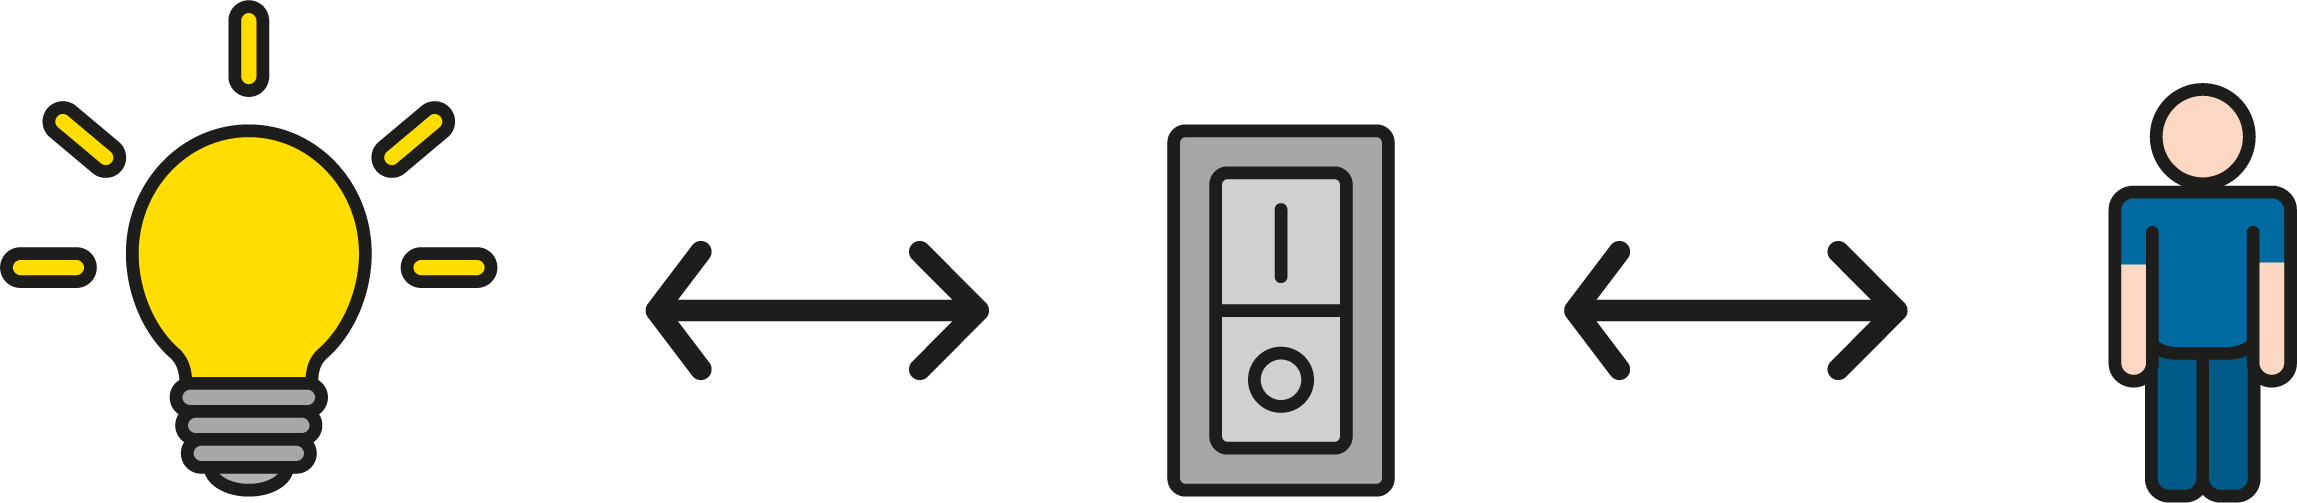
\includegraphics[width=13.5cm]{img/1_einleitung/HMI_Farbe}
	\caption{Grafische Darstellung eines \ac{HMI}}
	\label{fig:gra_hmi}
\end{figure}

Es gibt deutlich komplexere \acp{HMI} als einen Lichtschalter, da es deutlich komplexere Maschinen gibt und die Komplexität immer weiter steigt. Einige Maschinen lassen sich ohne aufwendige Interfaces nicht mehr bedienen. Das setzt allerdings auch ein immer größeres Hintergrundwissen derer Menschen voraus, welche die Maschinen bedienen.\\

\subsection{Geschichte von HMIs im automotive Bereich}
Die Geschichte und Entwicklung von \acp{HMI} wird in diesem Kapitel anhand von verschiedenen Beispielen erläutert. Wie im vorherigen Teil beschrieben, ist etwa ein Lichtschalter eine sehr einfache Schnittstelle. In Fahrzeugen wurden schon immer Schnittstellen benötigt, allerdings haben sich die Anzahl und die Umsetzung über die Jahre stark verändert.\\

Während den Anfängen des Automobils gab es unter anderem Schnittstellen, die heute nicht mehr benötigt werden. Dazu zählt unter anderem die Zündzeitpunktverstellung. Jedoch gab es auch damals Schnittstellen, die heute noch in gleicher oder ähnlicher Form existieren.\\

Schon beim allerersten Automobil war es nötig die Richtung der Bewegung zu bestimmen. Daher war auch im ersten Automobil von Carl Benz ein Lenkhebel verbaut. Ein Lenhebel zeigt an in welche Richtung gefahren wird. Durch drehen am Lenhebel lässt sich die Richtung ändern in die sich das Fahrzeug bewegt. Der Lenkhebel wurde später durch das Lenkrad ersetzt. Außerdem war es möglich die Geschwindigkeit zu verändern. Beim Benz Patent-Motorwagen Nummer 1 wurde die Abgabeleistung und damit die Geschwindigkeit noch mit einem Hülsenschieber geregelt. Heute wird das, über das Gaspedal und einen Bowdenzug, oder elektronisch geregelt.\\%cite wikipedia benz patent motor wagen nummer 1

Mit der Zeit veränderten sich die Schnittstellen und neue Schnittstellen kamen hinzu. Nicht mehr benötigte Schnittstellen wurden entfernt und die wichtigen Schnittstellen wurden immer weiter verbessert. Durch die Verbreitung des Automobils wurde es voller auf den Straßen. Die Fahrzeuge erreichten höhere Endgeschwindigkeiten und die Sicherheit rückte in den Fokus. Trotz der im Durchschnitt geringeren Verkehrsdichte im Vergleich zu heute, häuften sich die Unfälle. Da die Fahrer unter anderem die Geschwindigkeit nicht richtig einschätzen konnten. Im Jahr 1902 wurde der Wirbelstrom-Tachometer von Otto Schulze entwickelt. Diese Art Tachometer zeigte den Fahrern die Geschwindigkeit ihres Fahrzeugs an.\\ %cite wikipedia tacho

Der Tachometer war nicht das letzte Instrument, dass Einzug in die Fahrzeuge gehalten hat. Immer mehr Instrumente halfen dem Fahrer sein Fahrzeug zu steuern und zu überwachen. Früher wurden größtenteils Instrumente entwickelt die dem Fahrer wichtige Informationen vermittelten. Darunter zum Beispiel die Kilometer-Anzeige, so konnte festgestellt werden wie groß die Reichweite des Fahrzeugs ist. Eine Drehzahl-Anzeige hilft dabei den richtigen Gang zu wählen. Diese und weitere Anzeigen befinden sich heute größtenteils direkt hinter dem Lenkrad. Die Position, direkt hinter dem Lenkrad, liegt im Sichtfeld des Fahrers und sorgt dafür, dass die wichtigsten Informationen ohne große Ablenkung vom Fahrer erfasst werden können.\\
 
Diese Anordnung von Instrumenten nennt sich Instrument Cluster (Kombiinstrument) und hat sich bis heute etabliert. Je nach Fahrzeughersteller unterscheiden sich die Instrument Cluster in einigen wenigen Punkten. Die Grundfunktionen sind allerdings bei allen Herstellern gleich.\\

%Hinführung zum Thema
\subsection{Hinführung zum Thema}
Diese Arbeit befasst sich mit der \titleDocument. Instrument Cluster bündeln die für den Fahrer wichtigen Informationen und stellen diese grafisch dar. Dazu zählen zum Beispiel das Tachometer, Drehzahlanzeige, Tankanzeige und die Kühlwassertemperatur. Je nach Ausstattungsvariante sind unter anderem noch verschiedene Multimedia-Funktionen verfügbar. Von Freisprechanlage, über Rückfahrkamera bis hin zur Navigation sind den Funktionen nahezu keine Grenzen gesetzt.\\

%welche fahrzeugklassen gibt es grob?
Instrument Cluster sind in nahezu allen Fahrzeugklassen vertreten und bestehen heute zum überwiegenden Teil aus einem oder mehreren Displays. Da sich das Kombiinstrument größten teils hinter dem Lenkrad befindet wird die Steuerung mit Tastern und Drehgebern gelöst. Tesla hingegen setzt auf ein Instrument Cluster in der Mittelkonsole, welches sich ausschließlich durch Touch bedienen lässt.\\

% Hier Beispielbild
% Quelle? BEG?

\begin{figure}[htb]
	\centering
	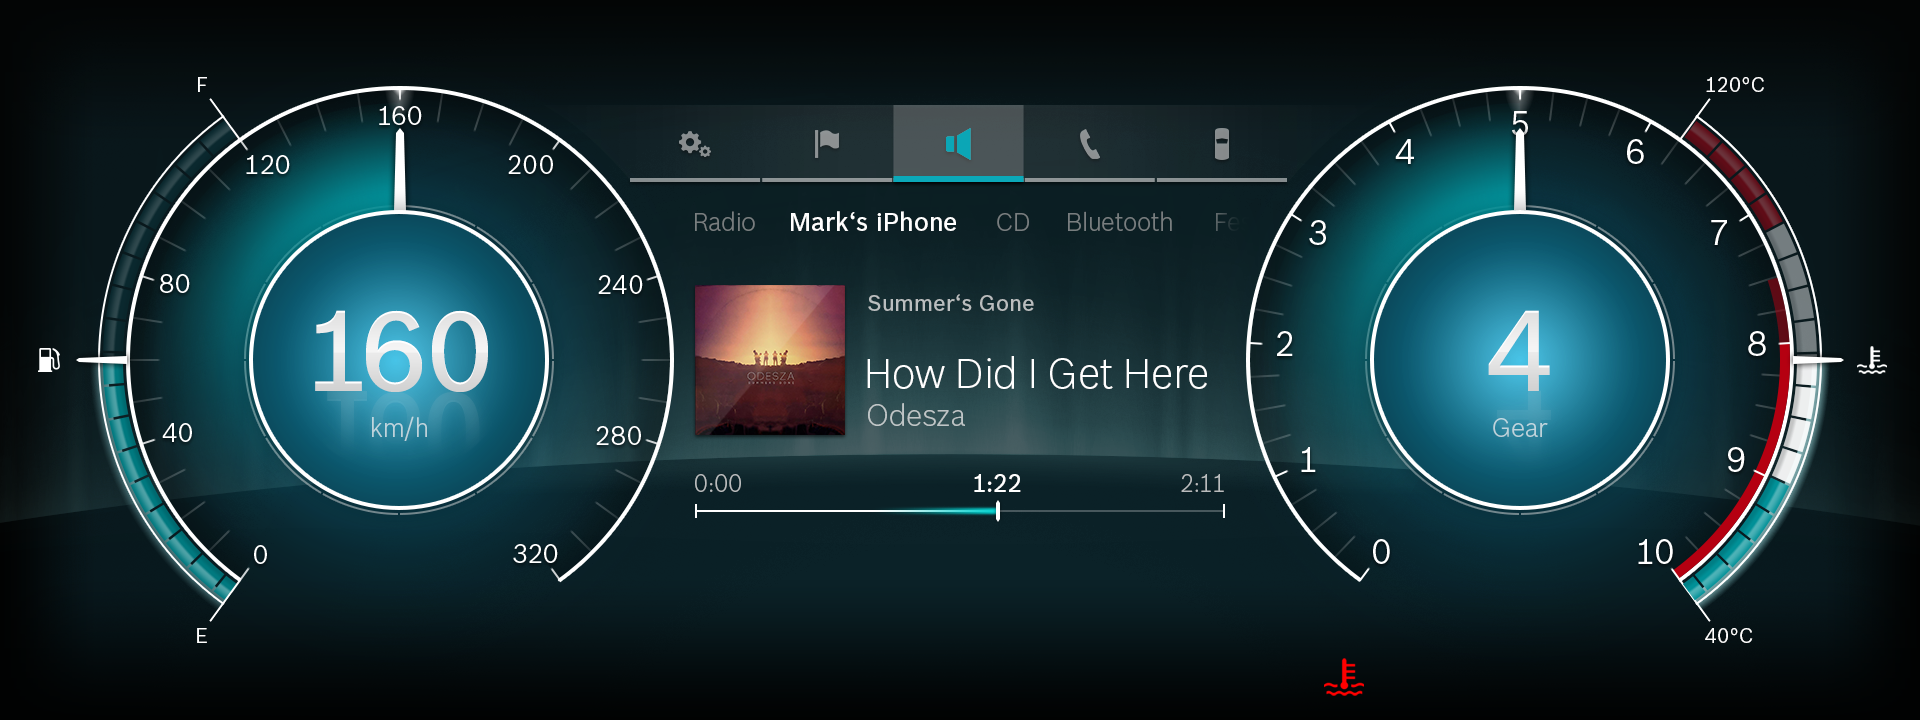
\includegraphics[width=\textwidth]{img/1_einleitung/beispielHMI}
	\caption[Beispielhaftes Instrument Cluster]{Beispielhaftes Instrument Cluster \cite{bosch}}
	\label{fig:hmi}
\end{figure}

% Erklärung zum Bild
Als Beispiel dient Abbildung \ref{fig:hmi}, dort ist eine Standardszene eines Kombiinstruments dargestellt. Links ist der Tachometer zu sehen. Die Geschwindigkeit wird einmal analog als Zeigerinstrument nachgebildet und einmal digital angezeigt. Links daneben befindet sich die Tankanzeige. Die rechte Seite zeigt die aktuelle Drehzahl und den aktuellen Gang an. Rechts daneben wird die Kühlwassertemperatur angezeigt. Die Mitte wird ausgefüllt von Multimedia-Funktionen wie Musik, Telefon und Navigation.\\

% Thema weiter erklären ->Entwicklung HMI Konzept
In der vorliegenden Arbeit, wird zunächst ein Architektur-Konzept entwickelt. Die Entwicklung dieses Konzepts umfasst die Recherche des aktuellen Stands sowie die Erstellung eines neuen Software-Architektur-Konzepts. Im Fokus stehen hierbei zum einen ein geringer Entwicklungs- und Kostenaufwand und zum anderen ein möglichst hohes Maß an Flexibilität. Der Entwicklungsaufwand, sowie die -kosten können durch standardisierte Software verringert werden. Diese Art der Software muss gleichzeitig einen großen Kreis an Kunden ansprechen um profitabel zu sein. Im Gegensatz dazu steht die individuelle Softwarelösung. Diese Art der Software erhöht Aufwand und Kosten. Deshalb gilt es ein Konzept zu finden das beide Ansätze optimal vereint.\\

%Architektur entwickeln
Eine Architektur zu entwickeln, ist ein umfangreicher Prozess. Damit dieser Prozess gelingt, müssen einige Dinge beachtet werden. So existieren zum Beispiel eine Reihe von ISO Normen die sich mit der Bewertung der Qualität von Software auseinandersetzen. Zudem gibt es verschiedene Designmöglichkeiten die sich gegenseitig ausschließen.\\

% Umsetzung des Konzepts
Für die Umsetzung des Konzepts gilt es als erstes eine grobe Architektur festzulegen. Danach muss die Entwicklungsumgebung ausgewählt werden. Die Software soll in jedem Fall wiederverwendbar sein, daher soll die Software möglichst aus Entwurfsmustern bestehen. Entwurfsmuster helfen, Software in einzelne wiederkehrende Muster aufzuteilen.\\

Die Auswahl an Entwicklungsumgebungen ist groß, daher muss hier eine Auswahl getroffen werden. Anschließend werden die Entwicklungsumgebungen getestet und müssen bewertet werden. Zur Wahl stehen hier CGI Studio, Storyboard und Qt. CGI Studio ist das aktuelle Entwicklungstool bei der Bosch Engineering GmbH. Hier soll eine mögliche Alternative gefunden werden, da zum einen die Einarbeitungszeit sehr hoch ist und zum anderen sind einige Funktionen sehr fehleranfällig. Sobald das Konzept fertig und die Entwicklungsumgebung gefunden ist, soll eine Prototypen-Software entwickelt werden. Damit soll gezeigt werden wie das Konzept umgesetzt werden kann.\\

%Ziele definieren
Das Ziel der Arbeit besteht zum einen aus der Erarbeitung einer Software-Architektur. Die Architektur soll den Entwicklungsaufwand für zukünftige Projekte zu reduzieren. Zum anderen muss ein dafür passendes Framework gefunden werden, mit dem die Architektur umgesetzt werden kann.\\


% \newpage
% % !TEX root = Hauptdatei.tex
\section{Stand der Technik}\label{standDerTechnik}

Im folgenden Kapitel wird der aktuelle Stand der Technik bei der \ac{BEG} beschrieben. Es wird erläutert mit welchen Tools und Vorgehensweisen bisherige Projekte umgesetzt wurden.\\

\subsection{Kundenorientierte Software}
Der erste Ansatz ist die kundenorientierte Software. Das heißt, für den Kunden wird eine komplett angepasste Software entwickelt. Bisher wurde dazu auf Plattformen von großen Automobilherstellern zurückgegriffen. Die Plattformen bestehen aus Hardware und Software. Plattformen sind fertige Systeme die immer wieder verwendet werden können. Zunächst wird geprüft welche Hardware am Besten zu den Anforderungen des Kunden passt, die passendste Hardware wird übernommen. Die dazugehörige \ac{HMI} wird allerdings komplett neu entwickelt.\\

Die Entwicklung einer komplett neuen \ac{HMI} erfordert einen hohen Kosten- und Entwicklungsaufwand. Daher lohnt sich dieser Ansatz nur für große Kunden. Ein großer Kunde kann die hohen Entwicklungskosten auf die Masse an Fahrzeugen aufteilen, dadurch sinken die Kosten pro Fahrzeug. Kleiner Kunden haben mit dieser Vorgehensweise Schwierigkeiten. Bei einer geringen Stückzahl steigen die Kosten pro Fahrzeug enorm. Deshalb ist diese Lösung für kleine Kunden mit wenig Budget eher weniger geeignet. Kunden die weniger Geld ausgeben wollen, fokussieren sich mehr auf eine modulbasierte Lösung.\\
  
\subsection{Modulbasierte Software}
Der zweite Ansatz ist die modulbasierte Software. Eine modulbasierte Software heißt, es gibt viele vorgefertigte Bestandteile einer Software aus denen der Kunde wählen kann. Allerdings bedeutet das auch, dass der Kunde wenig bis gar nicht personalisieren kann. Eine modulbasierte Software lässt sich nur geringfügig auf die Belange des Kunden anpassen. Das hat aber den Vorteil, dass diese Lösung sehr kostengünstig ist und nur einen geringen Entwicklungsaufwand erfordert.\\
 
In diesem Kapitel wird auf eine von Bosch entwickelte, modulbasierte Software, eingegangen. Bosch bietet dem Kunden hier die Möglichkeit zwischen drei Ausbaustufen zu wählen. Je nach Ausbaustufe lassen sich mehr oder weniger Komponenten, vom Kunden anpassen.\\

Als Betriebssystem wird Yocto Linux für eingebettete Systeme verwendet. Yocto Linux ist ein Opensource-Projekt das die individuelle Erstellung eines Linux Betriebssystem ermöglicht. Das Betriebssystem kann auf die eigenen Bedürfnisse angepasst werden.\\

Die Plattform ist aufgeteilt in drei Ausbaustufen.
\begin{itemize}
	\item Standard
	\item Customized Standard
	\item Customized 
\end{itemize}

Die Standard-Ausbaustufe lässt sich nur in sehr begrenztem Umfang anpassen. In Abbildung \ref{fig:standard} sind die einzelnen Module zu sehen. Blau zeigt die Möglichkeiten zur Anpassung. Je geringer der Blauanteil in einem Kasten, desto weniger kann angepasst werden. In der Standard-Ausbaustufe werden nur Grafiken ausgetauscht, der Rest bleibt bei jedem Kunden gleich. Diese Stufe spricht vor allem kleine Kunden an, da sie die kostengünstigste Stufe ist.

\begin{figure}[htb]
	\centering
	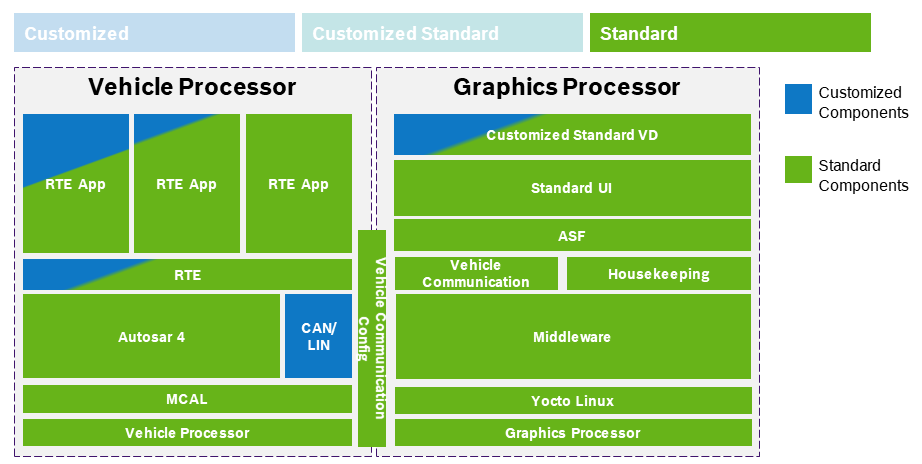
\includegraphics[width=\textwidth]{img/2_stand_der_technik/STICC_3_neu}
	\caption[Architektur der Standard-Ausbaustufe]{Architektur der Standard-Ausbaustufe \cite{bosch}}
	\label{fig:standard}
\end{figure}

Die Customized-Standard-Ausbaustufe bietet etwas mehr Auswahlmöglichkeiten für den Kunden. Trotzdem sehen sich die Endergebnisse sehr ähnlich, wie Abbildung \ref{fig:cu_st} zeigt, ist der Blauanteil etwas größer. Dadurch ergibt sich für den Kunden eine etwas größer Anpassungsmöglichkeit. So kann er in dieser Ausbaustufe das Visual Design komplett anpassen und zum Teil auch die Standard UI. \\

\begin{figure}[htb]
	\centering
	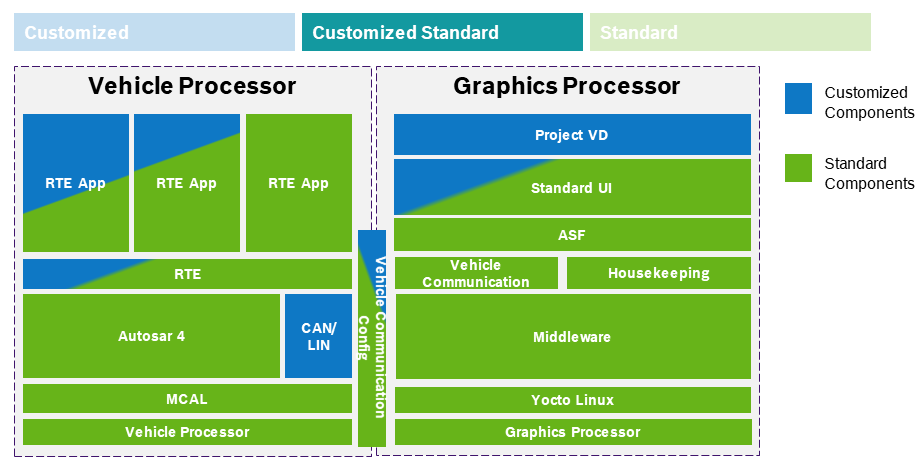
\includegraphics[width=\textwidth]{img/2_stand_der_technik/STICC_2_neu}
	\caption[Architektur der Customized-Standard-Ausbaustufe]{Architektur der Customized-Standard-Ausbaustufe \cite{bosch}}
		\label{fig:cu_st}
	\end{figure}
	 
Die letzte Ausbaustufe, in Abbildung \ref{fig:customized} zu sehen, bietet für den Kunden die größtmögliche Anpassungsmöglichkeit. Die Customized-Ausbaustufe ist bezüglich der Entwicklung - und damit auch der Kosten - die aufwendigste Stufe. Diese Stufe wird vor allem von den großen Herstellern gewählt. Zum einen um sich von den Wettbewerbern abzuheben und zum anderen, weil durch die Skaleneffekte der Kostenanteil beim Einzelfahrzeug geringer ausfällt.

\begin{figure}[htb]
	\centering
	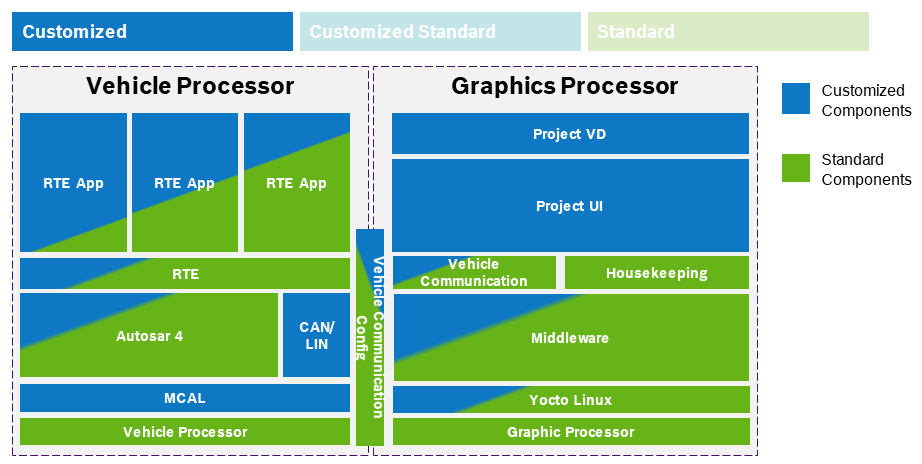
\includegraphics[width=\textwidth]{img/2_stand_der_technik/STICC_1_neu}
	\caption[Architektur der Customized-Ausbaustufe]{Architektur der Customized-Ausbaustufe \cite{bosch}}
	\label{fig:customized}
\end{figure}

Die bisherigen Nachteile der aktuellen Umsetzung sind zum einen die Hochlaufzeit und zum anderen die eingeschränkten Anpassungsmöglichkeiten.\\

\subsection{CGI Studio}
Die \ac{HMI}-Entwicklung erfolgt mit CGI Studio. CGI Studio ist das aktuelle Standardtool innerhalb der \ac{BEG}.\\

\glqq CGI Studio ist eine skalierbare und hardwareunabhängige Softwareplattform. Die offene Architektur ermöglicht eine tiefe Integration und Automatisierung. Die Software erlaubt die Erstellung von brillanten und anpassbaren \acp{HMI} aller Art für den Automobilbereich und darüber hinaus.\grqq{} \cite{canderaFAQ}\\

CGI Studio wird von dem österreichischen Unternehmen SocioNext entwickelt. Das Tool funktioniert nach dem \ac{WYSIWYG}-Prinzip. Die Grafiken werden importiert und können dann in den Editor gezogen werden.\\

% Was ist MVC
% Model, View, Controller erklären & was von CGI wo dazu gehört
% Bisschen zur Umsetzung
\subsection{Model-View-Controller}
Der \ac{MVC} ist ein Entwurfsmuster, dass die Daten, die Handhabung der Daten und die Anzeige der Daten trennt. Das Model empfängt Nachrichten über \ac{CAN} vom \ac{KSS} und sendet Daten an den Controller oder die View. Die empfangenen Nachrichten sind entweder Daten des Fahrzeugs oder eine Kontrollanweisung. Daten können zum Beispiel, Geschwindigkeit, Temperatur oder Drehzahl, sein und werden direkt an den Viewcontroller innerhalb der View geschickt. Eine Kontrollanweisung könnte ein Tastendruck oder das Drehen eines Drehencoders sein. Zwischen Model und Viewcontrollern existiert noch ein Zustandsautomat der regelt welcher Screen wann angezeigt wird. Der Controller entscheidet, was angezeigt wird und die View entscheidet, wie etwas angezeigt wird.\\

\begin{figure}[htb]
	\centering
	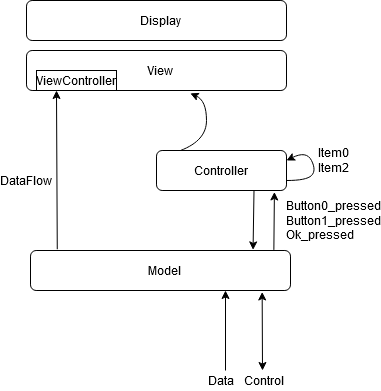
\includegraphics[width=10cm]{img/2_stand_der_technik/ModelViewControler}
	\caption{\acs{UML}-Diagramm eines Model-View-Controllers}
	\label{fig:mvc}
\end{figure}

\newpage

\subsubsection{Model}

% Quellen
% https://inside-docupedia.bosch.com/confluence/display/hmicore/Courier-based+HMI+Architecture

Die Model Komponente kümmert sich um das Empfangen und Weiterleiten von Nachrichten. Nachrichten, welche von dem \ac{KSS} kommen, müssen an die richtigen Empfänger verteilt werden. Ein Knopfdruck beispielsweise muss an den Controller geleitet werden um einen neuen Screen darzustellen. Eine Änderung der Geschwindigkeit muss jedoch an die View geschickt werden, damit der neue Wert in der Szene angezeigt wird.\\

Das Model stellt die, für die \ac{HMI}, relevanten Daten bereit. Das Model aktualisiert dann den Controller und die View mit Hilfe des Beobachtermusters. Das Model besitzt keine Abhängigkeiten gegenüber der Plattform. Im Model werden die Daten auf Plausibilität geprüft und wenn nötig in eine andere Einheit umgerechnet. Anschließend werden die Daten der View oder dem Controller zur Verfügung gestellt.\\

In CGI Studio wird das Model durch weitere Komponenten dargestellt, die sich um die korrekte Verteilung kümmern (z.B. Courier-Klasse). Diese sind im Folgenden nicht relevant und werden entsprechend nicht näher beschrieben.\\

\subsubsection{View}

Die View stellt die Daten aus dem Model grafisch dar. Die einzelnen Instrumente sind in Szenen aufgeteilt. Eine Szene kann zum Beispiel die Drehzahlanzeige oder die Außentemperaturanzeige sein. Die einzelnen Szenen werden im Scene Composer von CGI Studio erstellt. Die View fasst alle Szenen (Viewcontroller) zusammen, wie in Abbildung \ref{fig:scene} dargestellt. Für jede Szene existiert ein eigener Viewcontroller. Jeder Viewcontroller kann die Eigenschaften der zugehörigen Szene verändern. Aus den verschiedenen Szenen wird ein Screen erstellt. Der Screen wird dann auf dem Display gerendert dargestellt.\\

\begin{figure}[htb]
	\centering
	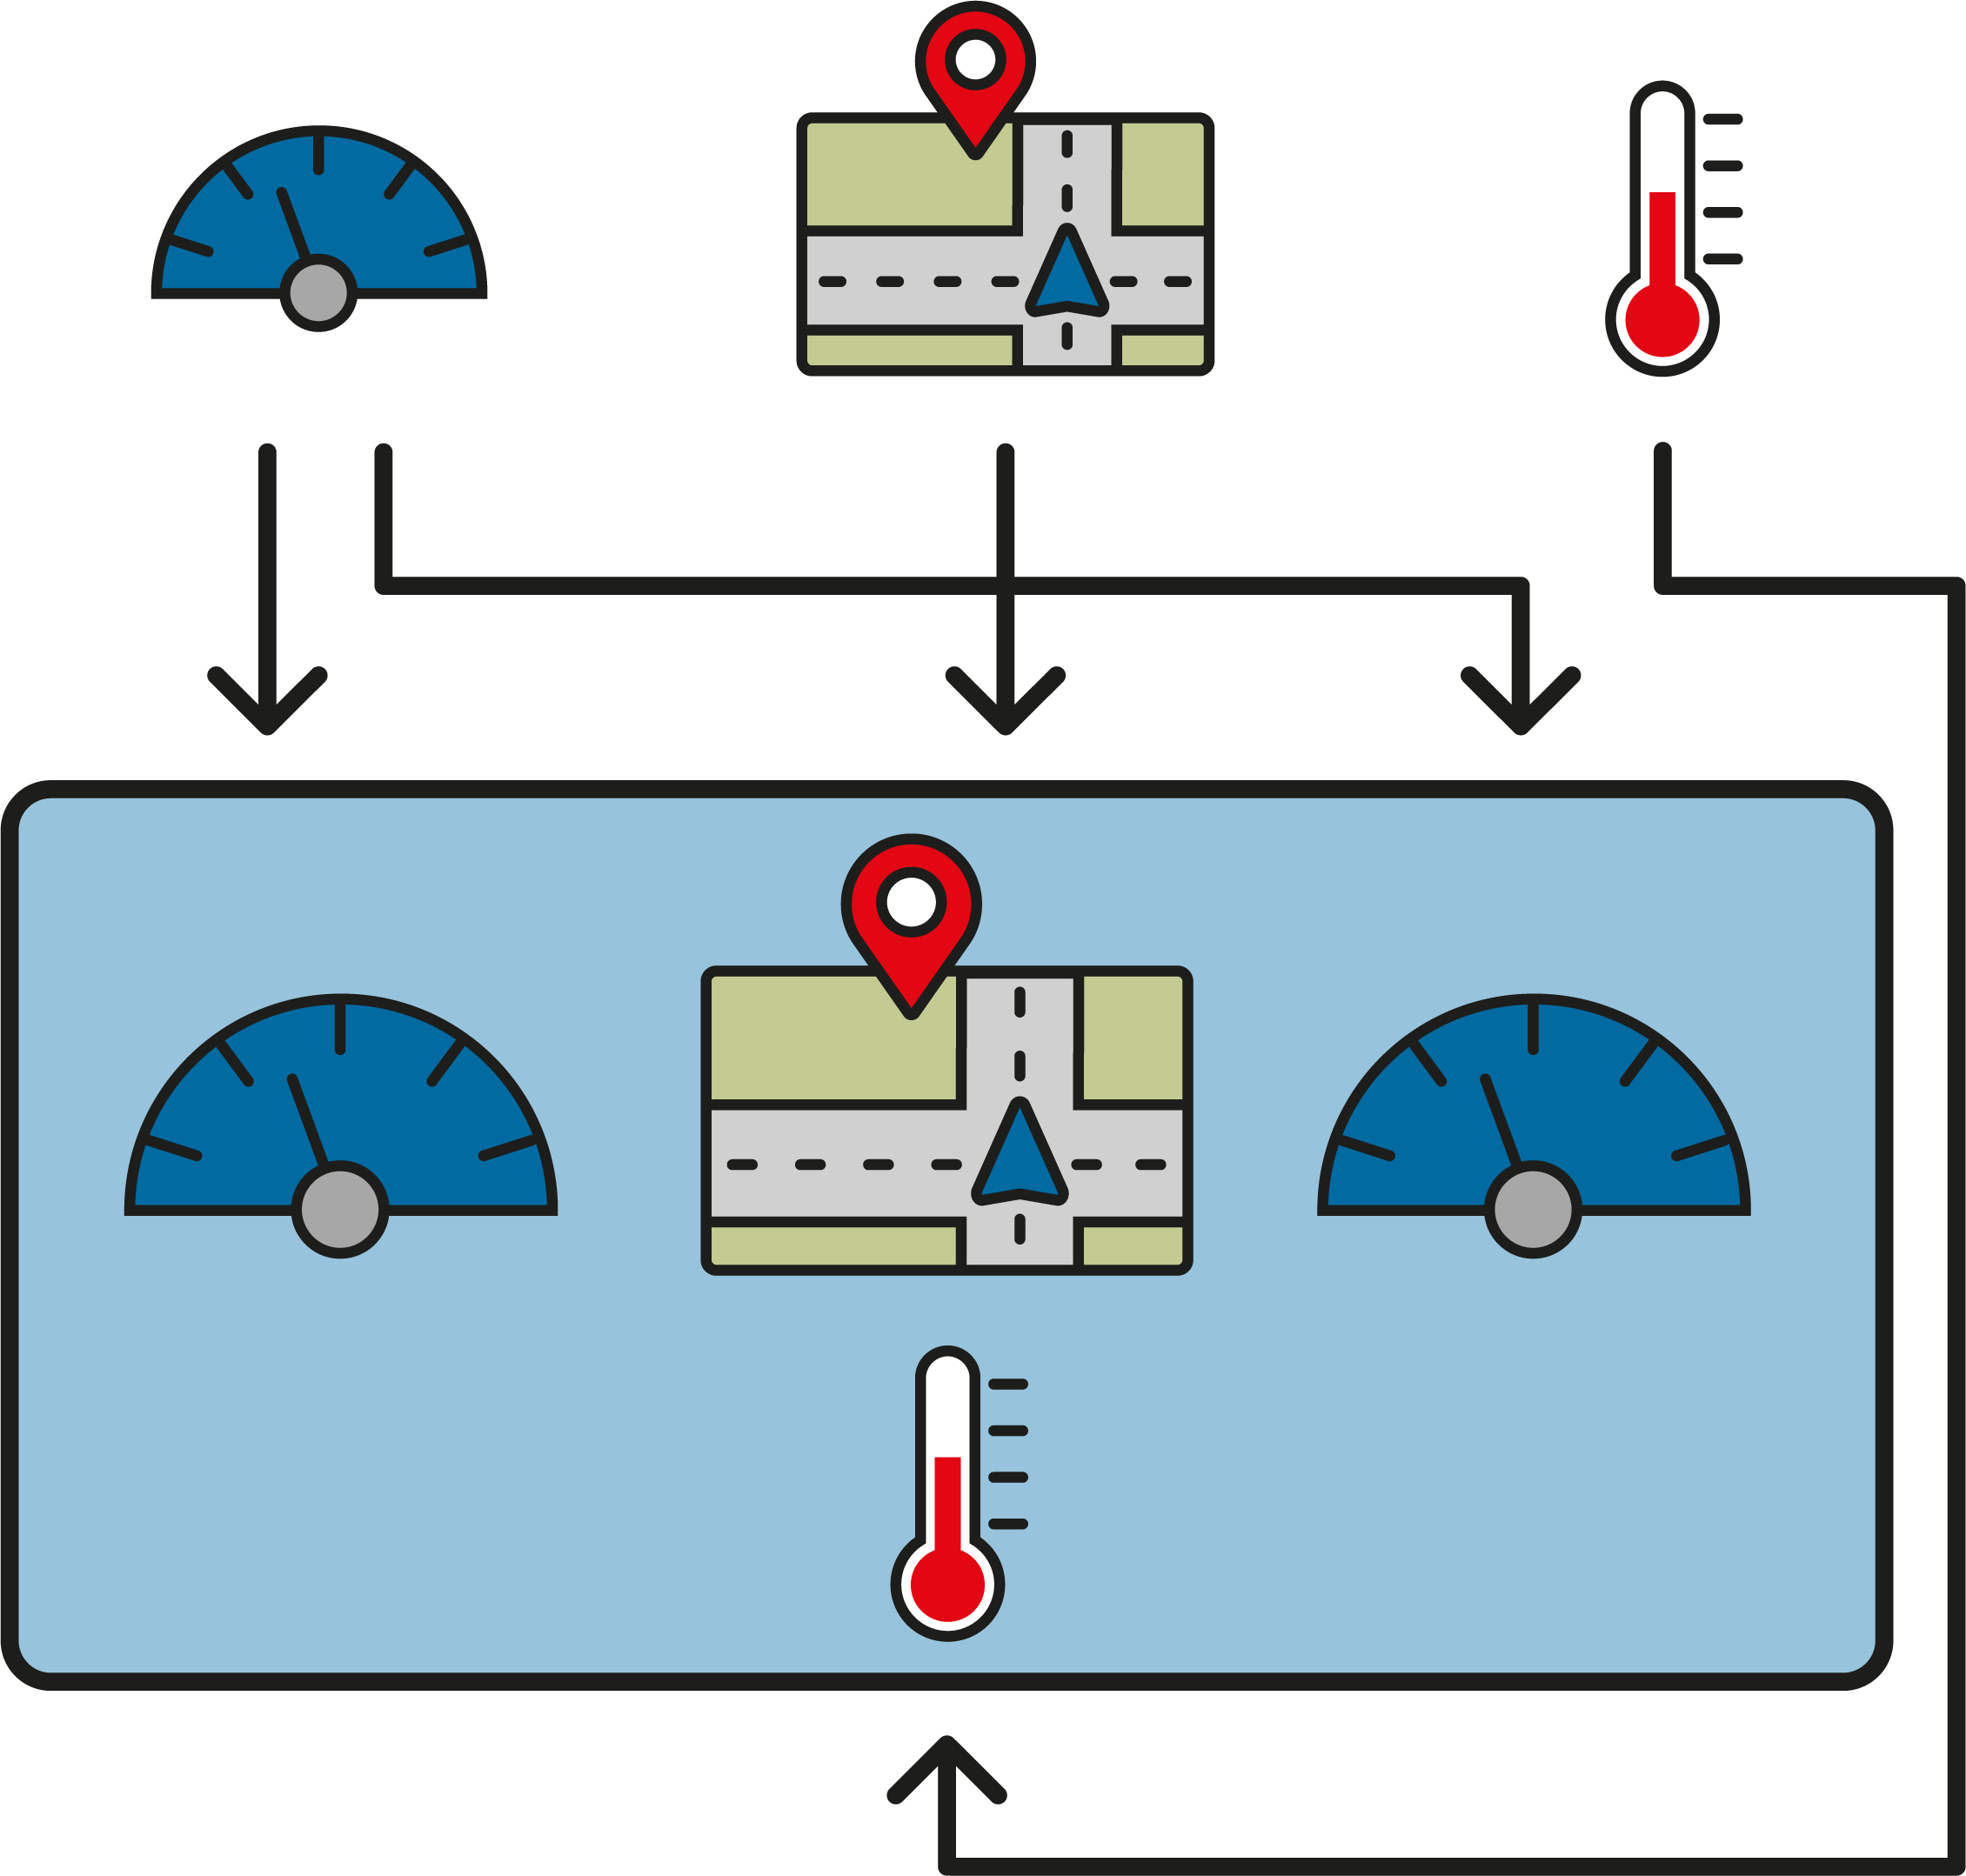
\includegraphics[width=14cm]{img/2_stand_der_technik/scene}
	\caption{Grafisches Beispiel einzelner Szenen zusammengesetzt zu einem Screen}
	\label{fig:scene}
\end{figure}




\subsubsection{Controller}
Der Controller reagiert auf Benutzerinteraktionen sowie Systemnachrichten und verändert basierend darauf die Anzeige des Kombiinstruments. Ein Controller besteht aus einem Zustandsautomaten. Jeder Zustand repräsentiert dabei eine definierte Anzeige auf dem Display. Durch einen Tastendruck oder andere Interaktionen wird zwischen den verschiedenen Zuständen gewechselt. Muss der Controller warten bis die View die alten Daten verarbeitet hat, benötigt der Controller ebenfalls einen Wartezustand.\\

\begin{figure}[htb]
	\centering
	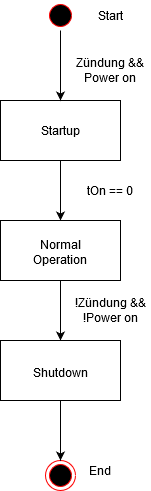
\includegraphics[width=4cm]{img/2_stand_der_technik/simple_statemachine}
	\caption{Beispielhafter Zustandsautomat eines Controllers}
	\label{fig:state}
\end{figure}

Abbildung \ref{fig:state} zeigt einen möglichen Zustandsautomat. Der abgebildete Zustandsautomat ist sehr simpel und enthält nur drei Zustände. Der erste Zustand \glqq Startup\grqq{} wird erreicht, wenn Klemme 15 geschlossen ist (Zündung an). Um hochzufahren benötigt das \ac{HMI} eine bestimmte Zeit, ist diese Zeit abgelaufen wechselt der Zustandsautomat in den \glqq Normal Operation\grqq{} Zustand. In diesem Zustand könnte zum Beispiel die aktuelle Geschwindigkeit und die Drehzahl des Motors angezeigt werden. Der Zustandsautomat verbleibt so lange in diesem Zustand bis Klemme 15 wieder geöffnet wird (Zündung aus). Durch diese Änderungen wechselt der Zustandsautomat in den \glqq Shutdown\grqq{} Zustand und beendet alle Funktionen.\\

Bisher wurden die Zustandsautomaten mit visualSTATE erstellt und dann dem Projekt hinzugefügt, mittlerweile bietet CGI Studio dafür eine eigene Lösung innerhalb des SceneComposer.\\
 

%bisschen mehr text
\subsection{Qualitätskriterien nach ISO 25010}\label{qualitaet}

Zu den Anforderungen werden in diesem Fall auch die Qualitätskriterien nach der ISO 25010 gezählt. Die ISO 250XX Reihe beschäftigt sich mit der Qualität und Bewertung von Software. Die ISO 25010 beschäftigt sich speziell mit dem Qualitätsmodell und passenden Leitlinien. Die ISO umfasst insgesamt 31 Qualitätskriterien, die sich auf acht übergeordnete Punkte verteilen. Eine Übersicht aus der ISO 25010 ist in Abbildung \ref{fig:Kriterien} dargestellt.\\

\begin{figure}[htb]
	\centering
	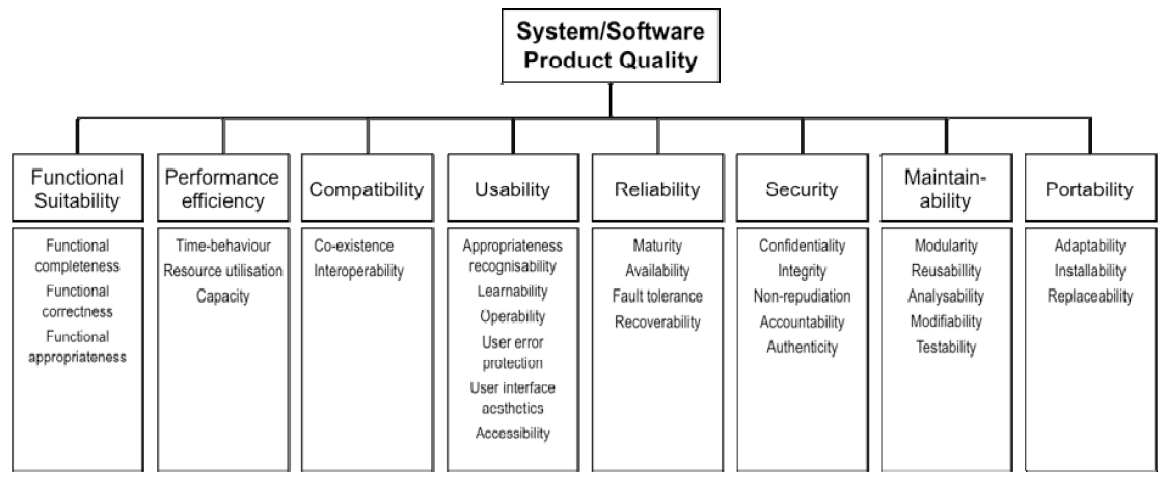
\includegraphics[width=\textwidth]{img/3_entwicklung_neues_kontept/Qualitaetskriterien}
	\caption[Qualitätskriterien aus der ISO 25010]{Qualitätskriterien aus der ISO 25010 \cite{iso25010}}
	\label{fig:Kriterien}
\end{figure}

Im Folgenden werden alle Qualitätskriterien kurz erläutert. \\
%Anschließend folgt eine Übersicht der Kriterien die im Hinblick auf das Architekturkonzept besonders relevant sind.\\

Die Functional Suitability beschreibt den Grad, in dem ein System Funktionen bietet, die den vorausgesetzten Bedürfnissen entsprechen. Dabei gibt die Functional completeness an wie weit die angegebenen Aufgaben und Benutzerziele durch den Funktionssatz abgedeckt werden. Im Gegensatz dazu zielt die Functional correctness darauf ab, in wie weit die richtigen Ergebnisse mit dem erforderlichen Grad an Präzision geliefert werden. Das letzte Kriterium die Functional appropriateness zeigt in wie weit Funktionen das Erfüllen bestimmter Aufgaben und Ziele erleichtert \cite{iso25010}.\\

Die Performance efficiency sagt etwas über die Performance relativ zu der Menge an Ressourcen unter gegebenen Bedingungen aus. Time-behaviour zielt dabei auf die Reaktions- und Bearbeitungszeit des Systems. Die Resource utilisation gibt die Anzahl und Arten der Ressourcen wieder (z.B. CPU, GPU, RAM, ROM). Die Capacity sagt aus, ob die Kapazität ausreicht (bsp. Anzahl an Menüs, Benutzter, usw.) \cite{iso25010}.\\

Die Compatiblity befasst sich mit dem Grad in dem ein System Informationen mit anderen Systemen austauschen kann, während sie die gleiche Hardware- oder Softwareumgebung teilen. Die Co-existence geht dabei darauf ein, in wie weit das Produkt die Ressourcen und Umgebung mit anderen Produkten teilen kann, ohne Performance zu verlieren. Bei der Interoperability wird beleuchtet, in wie fern zwei oder mehr Systeme Informationen austauschen und diese nutzen \cite{iso25010}.\\

Die Usability bezieht sich auf den Grad bis zu dem ein genutztes System, durch bestimmte Benutzter spezifizierte Ziele effektiv, effizient und zufriedenstellend erreicht. Dabei beschreibt die Appropriateness recognisability in wie weit der Nutzer erkennen kann, ob das System angemessen für seine Bedürfnisse ist, basierend auf den ersten Eindrücken und/oder mitgelieferten Dokumenten. Die Learnability zielt darauf ab wie einfach das Produkt oder System von bestimmten Nutzern erlernt werden kann um das Produkt oder System mit Wirksamkeit, Effizienz, Risikofreiheit und Zufriedenheit zu nutzen. Die Operability geht darauf ein, wie die Eigenschaften die Nutzung und Kontrolle vereinfachen. Die User error protection beschäftigt sich damit wie der Nutzer vor fehlerhaften Eingaben geschützt wird. Bei der User Interface aesthetics wird untersucht, ob die Interaktionen mit dem Benutzerinterface erfreulich und befriedigend sind. Die Accessibility analysiert, ob das Produkt von möglichst vielen Benutzern nutzbar ist \cite{iso25010}. \\


Die Reliability befasst sich damit, bis zu welchem Grad ein System, spezifizierte Funktionen unter bestimmten Bedingungen für eine definierten Zeitraum ausführt. Dabei beschäftigt sich die Maturity damit wie zuverlässig das Produkt bei normalem Betrieb ist. Die Availability beleuchtet, wie zugänglich das Produkt bei Bedarf ist und wie lange das Produkt ohne Fehler funktioniert. Die Fault tolerance überprüft, ob das System wie beabsichtigt funktioniert, trotz Hardware- oder Softwarefehler. Die Recoverability zielt darauf ab, ob das Produkt oder System im Falle einer Unterbrechung oder eines Ausfalls, die Daten die betroffen sind direkt wiederherstellen und den gewünschten Zustand des Systems wiederherstellen kann \cite{iso25010}.\\


Die Security interpretiert den Grad in dem ein System Informationen und Daten vor unberechtigten Zugriffen schützt. Die Confidentiality überprüft dabei, ob das System sicherstellt, dass nur autorisierte Benutzer Zugriff auf Daten bekommen. Die Integrity beschäftigt sich damit, ob das System unautorisierten Zugriff auf, oder Modifikation im Programm oder Daten verhindert. Non-repudiation erörtert wie verschiedene Aktionen nachgewiesen werden können. Die Accountability dagegen beschäftigt sich damit wie weit Handlungen eines Benutzers nachweisbar sind. Die Authenticity zielt darauf ab, ob die Identität einer Ressource nachgewiesen werden kann \cite{iso25010}\\


Maintainability gibt den Grad der Effektivität und Effizienz mit der ein System modifiziert werden kann an. Die Modularity beleuchtet, ob das Produkt in einzelne unabhängige Komponenten zerlegt und wie die einzelnen Komponenten zusammengefügt werden können. Die Reusability beschäftigt sich damit, wie weit ein Asset wiederverwendbar oder für andere Assets benutzbar ist. Die Analysability legt dar, wie effektiv und effizient beurteilt werden kann wie sehr andere Teile von einer beabsichtigten Änderung betroffen sind. Die Modifiability prüft, wie effektiv und effizient ein Produkt geändert werden kann ohne Auftreten von Mängeln, oder eine Verschlechterung der Produktqualität. Die Testability beschreibt, wie effektiv und effizient Testkriterien, für ein System, eingeführt und getestet werden können \cite{iso25010}.\\


Die Portability legt den Grad der Effektivität und Effizienz mit der ein System von einer Hard- oder Softwareumgebung in eine andere transferiert werden kann fest. Die Adaptability zielt darauf ab, ob sich ein System effektiv und effizient auf verändernde Hardware und Software anpasst. Die Installability beschäftigt sich damit, wie effektiv und effizient sich ein Produkt in einer speziellen Umgebung installieren und deinstallieren lässt. Die Replaceability legt dar, wie das System ein anderes System für den gleichen Zweck in der gleichen Umgebung ersetzt \cite{iso25010}.\\


%aus dem Buch Entwurfsmuster 
\subsection{Entwurfsmuster}
Bei der Entwicklung der Architektur soll auf Entwurfsmuster zurückgegriffen werden. Entwurfsmuster im Bereich Softwareentwicklung wurden maßgeblich von der \ac{GoF} etabliert. Die Gang of Four besteht aus den Softwareexperten Erich Gamma, Richard Helm, Ralph Johnson und John Vlissides, zusammen brachten sie 1994 das Buch Entwurfsmuster heraus.\\

Im Buch werden 23 verschieden Entwurfsmuster eingeführt und ausführlich erklärt. Entwurfsmuster sollen dabei helfen, objektorientierten Code wiederverwendbarer zu gestalten. Die \ac{GoF} versucht immer wiederkehrende Entwurfsprobleme zu identifizieren und eine allgemeingültige Lösung dafür anzubieten. Die Entwurfsmuster wurden dabei in drei übergeordnete Kategorien eingeteilt, Erzeugungsmuster, Strukturmuster und Verhaltensmuster. Die Muster wurden zusätzlich noch eingeteilt in klassenbasiert oder objektbasiert. Daraus entsteht die Matrix aus Tabelle \ref{tab:pattern}.\\

\begin{table}[h]
	\centering
	\caption[Übersicht der Entwurfsmuster aus dem Buch Entwurfsmuster]{Übersicht der Entwurfsmuster aus dem Buch Entwurfsmuster \cite{noauthor2011EntwurfsmusterElemente} }
	\label{tab:pattern}
	\begin{tabular}{|c|c|c|c|}\cline{2-4}
		\multicolumn{1}{c|}{} 			& Erzeugungsmuster  & Strukturmuster 	& Verhaltensmuster	 \\ \hline
		\multirow{2}{*}{klassenbasiert} & Fabrikmethode  	&  Adapter 			& Interpreter		 \\
		 								&				 	&					& Schablonenmethode	 \\ \hline
		\multirow{9}{*}{objektbasiert} 	& Abstrakte Fabrik  & Adapter  			& Befehl			 \\
										& Erbauer			& Brücke			& Beobachter		 \\
										& Prototyp			& Dekorierer		& Besucher			 \\
										& Singelton			& Fassade			& Iterator			 \\
										&					& Fliegengewicht	& Memento			 \\
										&					& Kompositum		& Strategie			 \\
										&					& Proxy				& Vermittler		 \\
										&					&					& Zustand			 \\
										&					&					& Zuständigkeitskette\\ \hline
	\end{tabular} 
	
\end{table} 

Erzeugungsmuster beschäftigen sich mit der Erzeugung von Objekten. Strukturmuster beschäftigen sich mit der Zusammensetzung von Klassen. Verhaltensmuster beschäftigen sich damit wie Klassen und Objekte miteinander arbeiten. Die zweite Einteilung, bestimmt, ob das Muster sich auf Klassen oder Objekte bezieht \cite{noauthor2011EntwurfsmusterElemente}. \\

Die oben genannten Entwurfsmuster wurden 1994 veröffentlicht gehören heute aber immer noch zum Standard. Die Entwurfsmuster im Buch zielen größtenteils auf die Programmiersprache C++ ab, mittlerweile gibt es von anderen Softwareentwicklern eigens entwickelte Entwurfsmuster für andere Sprachen.\\

\subsection{Anforderungen an das HMI-Framework}
\label{use_cases}
%Use Cases
Das richtige Framework wird auf Basis von Use Cases ausgewählt. Diese Use Cases wurden 2017 für die Evaluation von \ac{CM} entwickelt und basieren auf den Funktionen von CGI Studio. Mit Hilfe der Use Cases soll festgestellt werden, ob ein \ac{HMI}-Framework, in Projekten, häufig benötigte Funktionen umsetzten kann.\\ 

Die Use Cases gliedern sich in sechs Kategorien. Innerhalb der Kategorien gibt es obligatorische und optionale Anforderungen. In den nachfolgenden Kapitel wird auf diese Kategorien näher eingegangen.\\

\begin{itemize}
	\item Cluster \ac{HMI}
	\item Visual Appearance
	\item Text- und Listenverhalten
	\item Externe Daten
	\item Überlappung
	\item Komplexes Listenverhalten
\end{itemize}

\subsubsection{Cluster HMI} 
%In der Kategorie Cluster \ac{HMI} liegt der Fokus auf den Grundfunktionen von Instrument Clustern. Dazu zählen Nadelinstrumente und Warnlampen. 

%In dieser Kategorie müssen mindestens zwei Nadelinstrumente umgesetzt werden. Die Nadeln jedes Instruments müssen jeweils von einem eigenen Eingangssignal ansteuerbar sein. Die Nadeln müssen über einen Nachleuchten-Effekt verfügen. Die Geschwindigkeit und Drehzahl müssen textbasiert angezeigt werden und die Einheit von \si[per-mode=repeated-symbol]{\kilo\meter\per\hour} in \si[per-mode=repeated-symbol]{mi\per\hour} änderbar sein. Ebenfalls muss ein Warnlampenset implementierbar sein, zu Warnlampen gehören unter anderem das Anschnall-Symbol oder die Motor-Kontrollleuchte. Die Symbole dafür sind nach ISO 2575:2010 standardisiert.\\

%neu
In der Kategorie Cluster HMI sollen die Standardfunktionen von Instrument Clustern überprüft werden. Es handelt sich dabei um Nadelinstrumente und Warnlampen.\\

Die Nadel des Nadelinstruments muss sich abhängig vom Eingangssignal bewegen. Sie soll einen Nachleuchten-Effekt besitzen, wenn sie sich bewegt. Neben der analogen Anzeige soll auch eine digitale Anzeige der Werte möglich sein. Eine textbasierte Einheitenanzeige muss umschaltbar zwischen Kilometer und Meile sein.\\

Zudem muss ein Warnlampenset implementierbar sein, zu Warnlampen gehören unter anderem das Anschnall-Symbol oder die Motor-Kontrollleuchte. Die Symbole dafür sind nach ISO 2575:2010 standardisiert.\\

%bild davon

\subsubsection{Visual Appearance}
\label{visual}
%neu
In dieser Kategorie sollen verschiedene visuelle Effekte überprüft werden. Dazu gehört zum Beispiel die Darstellung der \ac{ACC}-Funktion mit einem 3D-Modell eines Fahrzeugs.\\

Die \ac{ACC}-Funktion regelt den Abstand zum vorausfahrenden Fahrzeug über die Geschwindigkeit. Dadurch bremst und beschleunigt das Fahrzeug von selbst.\\

Ein 3D-Modell eines Fahrzeugs soll sich analog zum aktuellen Zustand entweder zum Betrachter hinbewegen oder wegbewegen. Das 3D-Modell stellt das vorfahrende Fahrzeug dar. Erhöht sich die Geschwindigkeit, muss der Abstand größer werden, da sich der Bremsweg vergrößert. Umgekehrt kann der Abstand kleiner werden, wenn sich die Geschwindigkeit verringert.\\

Neben dem 3D-Modell soll mit Zahlen der aktuell gehaltene Abstand in Metern und Sekunden angezeigt werden.\\

Außerdem soll es möglich sein, die Außenfarbe des Fahrzeugs, abhängig von einem Eingangssignal, zu ändern.\\


\subsubsection{Text- und Listenverhalten}
In dieser Kategorie müssen verschiedene Listen implementierbar sein, z.B. vordefinierte Listen mit ca. 20 Einträgen und lange Listen mit ca. 500 Einträgen. Die Listen müssen scrollbar sein. Zum einen muss von Eintrag zu Eintrag gescrollt werden können und zum anderen zehn Einträge auf einmal gescrollt werden können.\\

Von einer Liste soll in eine andere Liste gewechselt werden können und alle Texte müssen übersetzbar sein. Sprachen müssen anlegbar sein, bei einem Wechsel der Sprache müssen alle Texte übersetzt werden.

\subsubsection{Externe Daten}
Ein Video aus einer externen Videoquelle muss abspielbar sein

\subsubsection{Überlappung}
Mit einem eingehenden Anruf-Fenster muss die Möglichkeit zur Überlappung demonstriert werden. Das überlappende Fenster muss transparent sein, damit der Hintergrund sichtbar bleibt. Die im Hintergrund verbliebenen Instrumente sollen weiterhin aktualisiert werden.

\subsubsection{Komplexes Listenverhalten}
Hier soll eine Medienliste mit ca. 10000 Einträgen implementiert werden. Die Form der Liste muss eine Kurve sein. Die Größe der Elemente soll von der Position abhängig sein, in der Mitte das Größte nach außen hin werden die Elemente kleiner. Abhängig von der Länge der Texteinträge sollen die Listeneinträge unterschiedliche Größen und Formen haben. Das Scrollverhalten muss ein Pixel zu Pixel scrollen ermöglichen. Die Liste soll beim Stoppen des Scrollens einrasten, dabei sollen keine halben Elemente zu sehen sein. Jeder Eintrag besteht aus einem Text, Bild und Button. Jeder Eintrag soll einen Fortschrittsbalken haben der kontinuierlich aktualisiert wird. Am Ende der Liste muss eine Abprallen-Animation stattfinden.


% \newpage
% % !TEX root = Hauptdatei.tex
\section{Entwicklung des neuen Konzepts}\label{hauptabschnitt_3}

%Vorgehensweise
%	Qualitätskriterien/Anforderungen ISO 25010
%	Entscheidungsbewertung
%	Design Patterns/Architectural Patterns
%	Auswahl HMI Tool
%Konzeptionierung
%	Gewählte Architektur
%	Gewählte Patterns (MVC)


%Dieses Kapitel beschäftigt sich mit der Entwicklung des neuen \ac{HMI}-Konzepts. In den nachfolgenden Kapiteln wird der Prozess der Softwarearchitektur, für diese Plattform, beschrieben.
%Bei der Entwicklung des neuen Konzepts müssen zu aller erst die Anforderungen an die Software identifiziert werden. Mit Hilfe der Anforderungen kann nach und nach ein Konzept entwickelt werden. \\

Dieses Kapitel beschäftigt sich mit der Entwicklung des neuen \ac{HMI}-Konzepts. In den nachfolgenden Kapiteln wird das Konzept für eine Softwarearchitektur entwickelt. Dabei müssen zuerst die Anforderungen an die Software identifiziert werden. Mit diesen Anforderungen werden im Anschluss Entwurfsmuster bewertet und ausgewählt und anschließend ein Architektur-Konzept erstellt.\\


\subsection{Gewichtung der ISO25010-Kriterien}
\label{Bewertung der ISO25010-Kriterien}
Die ersten Architekturtreiber sollen mit einer Entscheidungsbewertung herausgefunden werden. Dazu werden die ISO 25010 Kriterien von verschiedenen Mitarbeitern unabhängig gewichtet. Für die Gewichtung werden die Kriterien in eine Gegenüberstellungsmatrix eingefügt, welche dann von erfahrenen Mitarbeitern abgewogen werden.\\
  

\begin{figure}[htb]
	\centering
	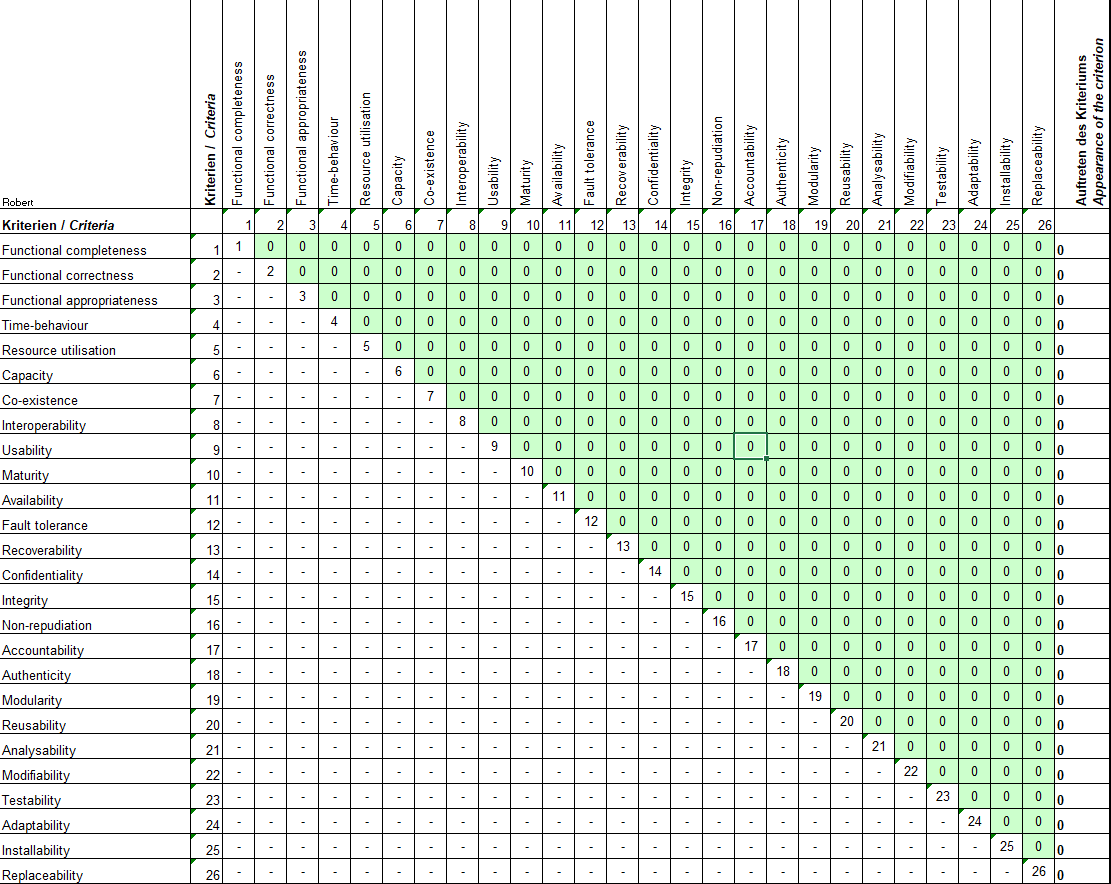
\includegraphics[width=\textwidth]{img/3_entwicklung_neues_kontept/Gewichtung}
	\caption{Gewichtungsmatrix der Qualitätskriterien nach ISO 25010}
	\label{fig:gewichtung}
\end{figure}
\newpage

Bei einer Gegenüberstellungsmatrix wird jedes Kriterium mit jedem anderen Kriterium verglichen.
Bei der Bewertung muss ausgewählt werden, welches Kriterium wichtiger ist. Die Matrix ist wie in Abbildung \ref{fig:gewichtung} aufgebaut. Die Kriterien stehen einmal in der vertikalen linken Spalte und einmal in der horizontalen Zeile in der gleichen Reihenfolge. In der Spalte daneben bzw. in der Zeile darunter bekommt jedes Kriterium eine fortlaufende Nummer, hier von 1 bis 26. In den Zellen in denen sich die gleichen Kriterien treffen wird direkt die Nummer des entsprechenden Kriteriums eingetragen, hier muss keine Entscheidung getroffen werden. Die eingetragenen Nummer bilden eine Diagonale durch die Matrix und teilt diese in zwei Hälften. Beide Hälften sind gleich, denn in beiden treffen sich jeweils alle Kriterien einmal. Daher muss nur die eine Hälfte ausgefüllt werden. Die obere rechte Hälfte wird zum Bewerten genutzt. Für die Bewertung muss dann in jede übrig gebliebene Zelle die Nummer des dominierenden Kriteriums eingetragen werden. Sind alle Zellen ausgefüllt ist in der rechten vertikalen Spalte das Ergebnis zu sehen. In dieser Spalte wird gezählt, wie oft ein Kriterium dominiert hat, das ist das Gewicht des Kriteriums.\\



\begin{table}[htb]
	\caption[Gesamtgewichtung]{Tabellarische Übersicht der Einzelgewichtungen der Qualitätskriterien}
	\label{tab:gewichtung}
	\centering
	\footnotesize
	\begin{tabular}{|l|c|c|c|c|c|}
		\hline
		                           & Architekt & SW-Entwickler & Kundensicht & Architekt & SW-Entwickler \\ \hline
		Functional completeness    &     5     &       1       &     15      &     1     &      11       \\ \hline
		Functional correctness     &    18     &      26       &     22      &    26     &      23       \\ \hline
		Functional appropriateness &     7     &      21       &     23      &    11     &      12       \\ \hline
		Time-behaviour             &    17     &      20       &     20      &    23     &      14       \\ \hline
		Resource utilisation       &    16     &      20       &     13      &    11     &       9       \\ \hline
		Capacity                   &     9     &      14       &     12      &     3     &       6       \\ \hline
		Co-existence               &     7     &      18       &      1      &     9     &      14       \\ \hline
		Interoperability           &     7     &       3       &     20      &    10     &      18       \\ \hline
		Usability                  &    10     &      17       &     16      &    15     &      14       \\ \hline
		Maturity                   &    24     &      16       &     16      &    24     &      24       \\ \hline
		Availability               &    18     &      14       &     18      &    24     &      26       \\ \hline
		Fault tolerance            &    24     &      22       &     16      &    13     &      22       \\ \hline
		Recoverability             &    23     &      13       &     14      &    16     &      22       \\ \hline
		Confidentiality            &    26     &      12       &     26      &    11     &      22       \\ \hline
		Integrity                  &    23     &      10       &     25      &    11     &      22       \\ \hline
		Non-repudiation            &     2     &       9       &      3      &     7     &      10       \\ \hline
		Accountability             &    14     &       9       &      4      &     6     &       6       \\ \hline
		Authenticity               &    16     &       8       &      5      &     6     &       9       \\ \hline
		Modularity                 &    15     &      24       &     10      &    18     &      17       \\ \hline
		Reusability                &    15     &       6       &      8      &    17     &      17       \\ \hline
		Analysability              &     5     &       7       &      5      &    19     &      11       \\ \hline
		Modifiability              &    11     &      23       &      9      &    20     &       9       \\ \hline
		Testability                &    18     &      24       &     24      &    22     &       5       \\ \hline
		Adaptability               &     7     &       5       &      3      &    21     &       5       \\ \hline
		Installability             &     2     &       4       &      7      &     4     &       2       \\ \hline
		Replaceability             &    12     &       3       &     15      &     3     &       1       \\ \hline
	\end{tabular}
\end{table}

Die Bewertung wurde insgesamt von fünf Personen aus unterschiedlichen Bereichen durchgeführt. Zu den verschiedenen Bereichen zählen zum einen zwei Software-Archi"=tekten, zwei Softwareentwickler und ein Akquisemitarbeiter für die Kundensicht. Diese Verteilung gibt eine gute Gesamtübersicht. Von der Systemplanung, über die Durchführung, bis hin zum Kunden sind dadurch alle Ansichten vertreten.
Das Ergebnis ist in Tabelle \ref{tab:gewichtung} dargestellt. \\
%Aus den unterschiedlichen Gewichtungen der Befragten wird eine Gesamtgewichtung berechnet. Hierzu wird der Durchschnitt genommen. Mit Hilfe der Gesamtgewichtung werden passende Entwurfsmuster ausgewählt die, die wichtigsten Qualitätskriterien weitstgehend erfüllen. Durch die Eingrenzung der möglichen Entwurfsmuster ist es leichter ein Architektur zu erstellen, da der Fokus auf ein paar wenige Entwurfsmuster gelegt werden kann.\\

Aus den Einzelgewichtungen der fünf Experten wird eine Gesamtgewichtung erstellt, dazu wird der Durchschnitt für jedes Kriterium berechnet. Das Ergebnis ist in Tabelle \ref{tab:gesamtgewichtung} zu sehen. Mit Hilfe dieser Tabelle können verschieden Entwurfsmuster bewertet werden.

\begin{table}[htb]
	\caption[Gesamtgewichtung]{Durchnittliche Gewichtung der ISO-Kriterien (sortiert nach Gewichtung)}
	\label{tab:gesamtgewichtung}
	\centering
	\small
	\begin{tabular}{|l|c|}
		\hline
		                           & Gesamt \\ \hline
		Functional correctness     &   23   \\ \hline
		Maturity                   &   21   \\ \hline
		Availability               &   20   \\ \hline
		Time-behaviour             &   19   \\ \hline
		Testability                &   19   \\ \hline
		Fault tolerance            &   19   \\ \hline
		Confidentiality            &   19   \\ \hline
		Recoverability             &   18   \\ \hline
		Integrity                  &   18   \\ \hline
		Modularity                 &   17   \\ \hline
		Functional appropriateness &   15   \\ \hline
		Usability                  &   14   \\ \hline
		Resource Utilisation       &   14   \\ \hline
		Modifiability              &   14   \\ \hline
		Reusability                &   13   \\ \hline
		Interoperability           &   12   \\ \hline
		Co-Existence               &   10   \\ \hline
		Capacity                   &   9    \\ \hline
		Authenticity               &   9    \\ \hline
		Analysability              &   9    \\ \hline
		Adaptability               &   8    \\ \hline
		Accountability             &   8    \\ \hline
		Replaceability             &   7    \\ \hline
		Functional Completeness    &   7    \\ \hline
		Non-Repudiation            &   6    \\ \hline
		Installability             &   4    \\ \hline
	\end{tabular}
\end{table}

%Einige der Kriterien sind für das Architektur-Konzept nicht relevant. Functional correctness 
\newpage
\subsection{Sammlung und Bewertung von Entwurfsmustern}
\label{Sammlung und Bewertung von Entwurfsmustern}
Damit Entwurfsmuster für die Architektur ausgewählt werden können, müssen zuerst Entwurfsmuster gesammelt und bewertet werden.\\

Bei der Recherche wurde der Fokus darauf gelegt, Entwurfsmuster im Zusammenhang mit den ISO-Kriterien zu finden. Da mit diesen Kriterien die Entwurfsmuster bewertet werden sollen. Aus der Recherche ergaben sich zwei wissenschaftliche Arbeiten die sich mit diesem Thema beschäftigten. Die erste Arbeit ist von 2006 mit dem Titel \glqq Towards a Maintainability Evaluation in Software Architectures \grqq \cite{towards_maintain} und die andere Arbeit von 2019 mit dem Titel \glqq Design Patterns for Software Evolution Requirements \grqq \cite{SW_evol_req}. Auf diese zwei Arbeiten wird in diesem Kapitel wesentlich Bezug genommen. Zusätzlich ergab die Recherche einen Report über sichere Entwurfsmuster, mit dem Titel \glqq Secure Design Patterns \grqq \cite{DoughertySecureDesign2009}.

\begin{figure}[htb]
	\centering
	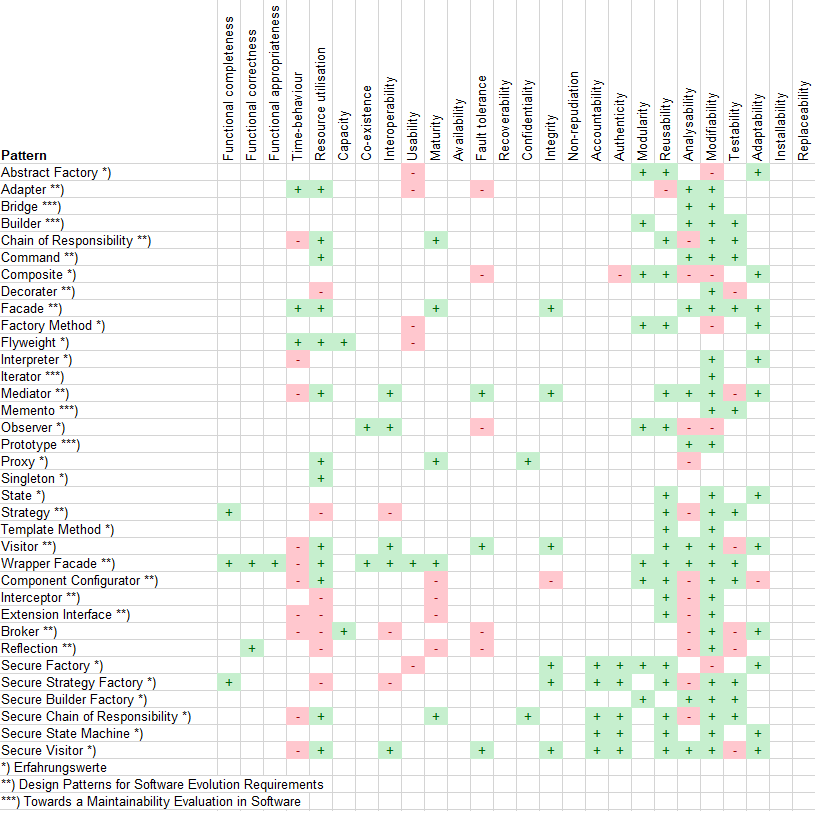
\includegraphics[width=14.5cm]{img/3_entwicklung_neues_kontept/Pattern_Sammlung_neu}
	\caption{Matrix der Entwurfsmuster und ISO-Kriterien}
	\label{fig:pattern_sam}
\end{figure}

Die ersten beiden Arbeiten beziehen sich vorwiegend auf die Standard-\ac{GoF}-Ent"=wurfs"=muster. Die letzte Arbeit hat die \ac{GoF}-Muster, unter dem Aspekt der Sicherheit, weiterentwickelt. Der Übersichtlichkeit wegen, wurden die Daten in eine Tabelle übertragen. Abbildung \ref{fig:pattern_sam} zeigt das Ergebnis. Die linke Spalte enthält alle gefundenen Entwurfsmuster in den Arbeiten und zusätzlich die \ac{GoF}-Entwurfsmuster, welche in keiner Arbeit erwähnt wurden. Die linke Spalte beinhaltet alle gefunden Entwurfsmuster. Die oberste Zeile enthält die ISO-25010 Kriterien. Dadurch ergibt sich eine Matrix, in der mit einem Plus, einem Minus, oder einer leeren Zelle das Entwurfsmuster in Bezug auf ein Kriterium bewertet werden kann. \\

\subsection{Auswahl Entwurfsmuster}
%Auswahl der Entwurfsmuster auf Basis der Entscheidungsbewertung

In diesem Kapitel werden die Ergebnisse aus Kapitel \ref{Bewertung der ISO25010-Kriterien} und Kapitel \ref{Sammlung und Bewertung von Entwurfsmustern} zusammengeführt. Die Entwurfsmuster werden in einer Matrix den ISO-Kriterien gegenübergestellt. Das Ergebnis ist eine Punktzahl für jedes Entwurfsmuster im Hinblick auf die ISO-Kriterien. Mit Hilfe der Punktzahl lässt sich feststellen, welche Entwurfsmuster am Besten zu der Gewichtung der Qualitätskriterien passen und worauf besonders geachtet werden sollte.\\

Die Punktzahl wird nach Gleichung 1 berechnet: Ein Minus in der Entwurfsmusterbewertung, heißt das Ergebnis der ISO-Bewertung wird mal eins genommen. Eine leere Zelle in der Entwurfsmusterbewertung, bedeutet das Ergebnis der ISO-Bewertung wird mal zwei genommen. Ein plus, heißt das Ergebnis der ISO-Bewertung wird mal drei genommen. Anschließend werden die Punktzahlen über alle Kriterien aufsummiert.\\

\begin{align}
	X &= \sum_{i=1}^{31} k_i\cdot z
\end{align}
\begin{align*}
	&X = \text{Punktzahl für Reihenfolge} \\
	&k_i = \text{Durchschnittsgewicht Kriterium 1 bis 31} \\
	&z = \text{1..3}
\end{align*}

Die Entwurfsmuster werden anschließend nach der erreichten Punktzahl sortiert. Daraus ergibt sich Tabelle \ref{tab:reihenfolge_pattern} mit der Reihenfolge der Entwurfsmuster.

\begin{table}[hp]
	\caption[Reihenfolge Entwrufsmuster]{Reihenfolge der Entwurfsmuster von oben (beste Punktzahl) nach unten (niedrigste Punktzahl)}
	\label{tab:reihenfolge_pattern}
	\centering
	\small
	\begin{tabular}{|l|c|l|}
		\hline
		Entwurfsmuster                 & Punktzahl & geeignet für      \\ \hline
		Command                        &   1520    & -                 \\ \hline
		Secure Chain of Responsibility &   1520    & -                 \\ \hline
		Wrapper Facade                 &   1504    & View              \\ \hline
		Memento                        &   1491    & View              \\ \hline
		Strategy                       &   1457    & View              \\ \hline
		Interpreter                    &   1446    & -                 \\ \hline
		Proxy                          &   1441    & View              \\ \hline
		Bridge                         &   1428    & View              \\ \hline
		Extension Interface            &   1393    & -                 \\ \hline
		Facade                         &   1376    & View              \\ \hline
		Secure Factory                 &   1302    & MVC               \\ \hline
		Secure Visitor                 &    790    & -                 \\ \hline
		Mediator                       &    773    & -                 \\ \hline
		Visitor                        &    773    & -                 \\ \hline
		Builder                        &    763    & -                 \\ \hline
		Secure Builder Factory         &    763    & -                 \\ \hline
		Chain of Responsibility        &    757    & -                 \\ \hline
		Secure Strategy Factory        &    757    & -                 \\ \hline
		Secure State Machine           &    756    & Controller        \\ \hline
		State                          &    739    & Controller        \\ \hline
		Flyweight                      &    732    & -                 \\ \hline
		Template Method                &    731    & -                 \\ \hline
		Prototype                      &    727    & -                 \\ \hline
		Iterator                       &    718    & -                 \\ \hline
		Singleton                      &    718    & Controller, Model \\ \hline
		Abstract Factory               &    714    & MVC               \\ \hline
		Adapter                        &    714    & -                 \\ \hline
		Factory Method                 &    714    & MVC               \\ \hline
		Observer                       &    714    & Model, View       \\ \hline
		Component Configurator         &    706    & -                 \\ \hline
		Compisite                      &    691    & -                 \\ \hline
		Interceptor                    &    687    & -                 \\ \hline
		Decorator                      &    685    & -                 \\ \hline
		Reflection                     &    659    & -                 \\ \hline
		Broker                         &    643    & -				   \\ \hline
	\end{tabular}
\end{table}
\newpage

In der Tabelle sind alle recherchierten Entwurfsmuster aufgelistet und sortiert nach der erreichten Punktzahl. In der rechten Spalte ist außerdem aufgeführt, für welchen Teil des Model-View-Controller das Entwurfsmuster geeignet ist. Da nicht jedes Muster zwangsläufig verwendet werden kann gibt es auch Zeilen ohne Eintrag. Im oberen Teil der Tabelle sind die meisten Entwurfsmuster der View zugeordnet. Daraus lässt sich schließen, dass der View den größten Teil der Aufmerksamkeit zu widmen ist.\\

\subsection{Architektur}
%Endgültige Architektur UML-Diagramme usw...

In diesem Kapitel wird die vorläufige Software-Architektur für das Proof-Of-Concept entwickelt. Die Architektur ist in diesem Fall noch nicht an die Eigenschaften von eventuellen \ac{HMI} Frameworks angepasst. Eine weitere Anpassung nach Auswahl des \ac{HMI}-Frameworks ist notwendig.\\

\glqq{}We need SMART Models, THIN Controllers, and DUMB Views\grqq{} \cite{mvc_wiki}. Dem entsprechend sollte der größte Teil der Komplexität im Model umgesetzt werden. Bei bisheriger Software lag der Hauptteil der Komplexität aber in den ViewControllern, also in der View. Der Controller sollte wirklich nur die Zustände verwalten und View sollte so wenig Komplexität beinhalten wie möglich. Das größte Augenmerk in der Entwicklung muss daher auf das Model gelegt werden. Der Controller und die View sollten schmal bleiben. Ziel sollte es sein, dass die Aufgaben im MVC-Muster strikt getrennt bleiben. Aufgrund des aktuell eingesetzten \ac{HMI} Frameworks konnte das \ac{MVC}-Muster nicht immer korrekt eingehalten werden.\\

In den folgenden Kapitel wird auf dieser Basis und den ausgewählten Entwufsmuster das Softwarearchitekturkonzept mit Hilfe von UML-Diagrammen erarbeitet.\\

\subsubsection{Model}
Das Model setzt sich aus dem Singleton-, Fabrik- und Beobachter-Entwurfsmuster zusammen. Das Singleton-Entwurfsmuster stellt sicher, dass eine Klasse nicht mehrfach instanziiert wird. Eine Mehrfachinstantiierung des Models würde Asynchronität der Daten und einen enormen Ressourcenverbrauch mit sich bringen. Das Singleton wird als abstrakte Klasse umgesetzt und das Model erbt von der Klasse Singleton. Die Fabrik kümmert sich um die Erstellung und Verwaltung vom Model. Die Verbindung zwischen Model und View bzw. Controller stellt das Beobachter-Muster her. Das Beobachter-Muster ermöglicht den Datenaustausch zwischen zwei oder mehr Objekten, verhindert aber gleichzeitig eine zu starke Kopplung der beteiligten Objekte. Die Implementierung des Beobachtermusters ist sehr stark vom verwendeten Framework abhängig.\\

Abbildung \ref{fig:model_diagram} veranschaulicht einen beispielhaften Entwurf des Models. Die in Abbildung \ref{fig:model_diagram} entworfenen Klassen sind als Beispiel zu verstehen und werden kundenspezifisch realisiert.\\

\begin{figure}[htb]
	\centering
	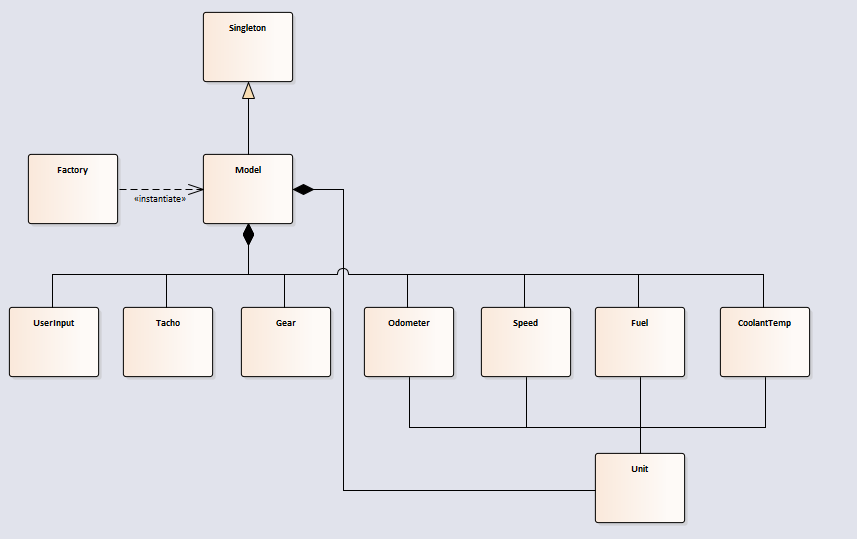
\includegraphics[width=\textwidth]{img/3_entwicklung_neues_kontept/model_diagram}
	\caption{UML-Diagramm des Model}
	\label{fig:model_diagram}
\end{figure}

In den einzelnen Modulen muss zunächst geprüft werden, ob erhaltene Werte plausibel sind. Nach der Plausibilisierung wird überprüft ob eine Umrechnung der Werte in eine andere Einheit notwendig ist. Nachdem alle Überprüfungen und Umrechnungen abgeschlossen sind, kann der Wert an die View weitergegeben werden.\\

Das Model soll so flexibel wie möglich sein und gleichzeitig Entwicklungsaufwand einsparen. Daher ist jede Klasse unabhängig von den anderen Klassen und kann jederzeit entfernt oder hinzugefügt werden. Der Vorteil von diesem Ansatz ist die hohe Modularität und die Möglichkeit große Teile des Models wiederzuverwenden. Dieser Ansatz kann im späteren Verlauf ein einfaches zusammenstellen des Models ermöglichen. Mit Hilfe eines Formulars könnten einzelne Module nach Kundenwunsch ausgewählt werden. Das Model wird dann durch ein Skript zusammengefügt und bereitgestellt.\\ 

\subsubsection{View}
Die konkrete Umsetzung der View hängt stark mit dem verwendeten HMI Framework zusammen und wird teilweise sogar vorgegeben.\\

Kapitel \ref{hauptabschnitt_4} beschäftigt sich mit der Evaluation dieser \ac{HMI} Frameworks und deren Einfluss auf eine Softwarearchitektur einer \ac{HMI}.\\

\subsubsection{Controller}
Der Controller besteht aus dem Singleton-, Zustand-, Fabrik- und Beobachter-Muster. Der Controller wird ebenfalls als Singleton realisiert, damit keine doppelten Zustände existieren und Ressourcen geschont werden. Im Controller ist jeder mögliche Zustand als konkrete Klasse realisiert. Die konkreten Zustände sind von der abstrakten Klasse Zustand abgeleitet. Die Fabrik kümmert sich auch hier um die Erstellung und Verwaltung des Controllers. Das Beobachter-Muster ist der Gegenpart zum Beobachter-Muster im Model. Das Model stellt die Daten bereit und der Controller verarbeitet die Daten und prüft einen möglichen Zustandswechsel. \\

Abbildung \ref{fig:controller_diagram} zeigt einen beispielhaften Entwurf eines Controllers. Die In Abbildung \ref{fig:controller_diagram} zu sehenden Zustände sollen als Beispiel verstanden werden und müssen kundenspezifisch durch konkrete Zustände ersetzt werden.\\

\begin{figure}[htb]
	\centering
	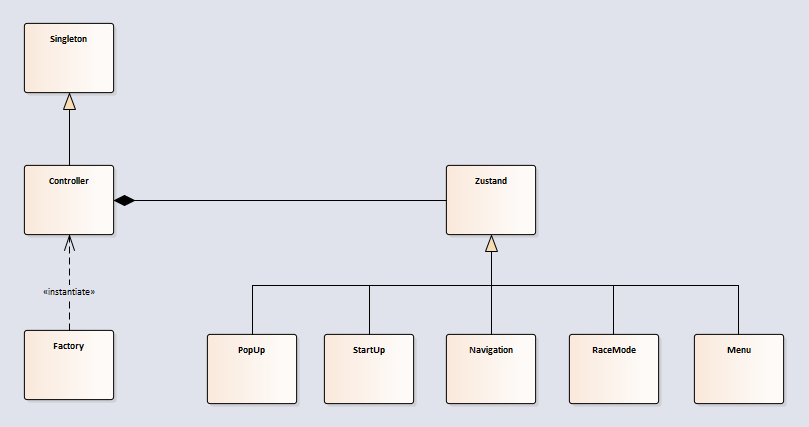
\includegraphics[width=\textwidth]{img/3_entwicklung_neues_kontept/controller_diagram}
	\caption{UML-Diagramm des Controllers}
	\label{fig:controller_diagram}
\end{figure}

Im Controller dürfen keine Berechnungen oder ähnliches stattfinden, es muss immer klar sein welcher Zustand der Aktuelle ist. Hier können ebenfalls Zustände beliebig hinzugefügt oder entfernt werden. Das ermöglicht auch hier, dass die Zustände in einem Formular ausgewählt werden können und anschließend durch ein Skript zusammengestellt wird.\\





% \newpage
% % !TEX root = Hauptdatei.tex
\section{HMI Frameworks}
\label{hauptabschnitt_4}

Im Jahr 2017 wurden bereits diverse HMI Frameworks seitens Bosch evaluiert. An verschiedene Anbieter von \ac{HMI}-Frameworks wurde eine Anforderungsliste geschickt. Die erfolgversprechendsten Anbieter wurden eingeladen um verschiedene Use Cases in ihrem Framework umzusetzen. Das Ergebnis der Evaluation war, dass CGI Studio die Anforderungen am Besten abdeckt.\\

In diesem Kapitel werden Storyboard und Qt erneut evaluiert. Qt wurde ausgewählt weil es bei der Evaluation 2017 gut abgeschnitten hat. Hauptkritikpunkt war die fehlende 3D-Unterstützung. Storyboard wurde als Gegenpart zu Qt ausgewählt. Storyboard versucht, im Gegensatz zu Qt, mit wenigen einfachen Funktionen den größtmöglichen Nutzen zu bieten. \\ 

\subsection{CGI Studio}
\label{cgi}
Das Tool CGI Studio wird aktuell von Bosch für die \ac{HMI}-Entwicklung eingesetzt. Aufgrund der langjährigen Nutzung sind viele Entwickler mit der Nutzung von CGI Studio vertraut. Im Rahmen dieser Arbeit gab es jedoch einige Schwierigkeiten CGI Studio zu testen. Der Scene Composer, in dem das HMI erstellt wird, lädt beim Start eine DLL-Datei. In dieser DLL-Datei, sind die Widgets und Controls hinterlegt. Das Verhalten und die Funktionen der Widgets und Controls müssen vorher in C++ programmiert werden. Anschließend wird eine DLL-Datei daraus erzeugt. Das ermöglicht für jedes Projekt eigene Widgets zu programmieren.\\

Diese Vorgehensweise birgt allerdings auch Probleme. Das Wissen zu den verschiedenen Widgets und Controls liegt sehr konzentriert bei den Projektbeteiligten. Zusätzlich gibt es für jedes Projekt eine eigene DLL-Datei, dadurch ist es sehr unübersichtlich, welche DLL-Dateien, welche Widgets beinhalten. Auch ob die Widgets noch aktuell sind, ist nicht ersichtlich.\\

Daher kam es vor allem zu dem Problem, dass der Scene Composer des öfteren abgestürzt ist. Das Problem war eine schlechte Fehlerbehandlung innerhalb eines Widgets. Es stellte sich im Nachhinein heraus, dass dieses Widget veraltet ist. Deshalb liegt der Fokus auf die zwei Mitbewerber Storyboard und Qt, welche in den folgenden Kapiteln beschrieben werden.\\ 


\subsection{Storyboard}
Storyboard wird von der Firma Crank Software Inc. entwickelt, die in Kanada ansässig ist. Storyboard basiert auf der Eclipse Entwicklungsumgebung.
\glqq Eclipse [...] ist ein quelloffenes Programmierwerkzeug zur Entwicklung von Software verschiedener Art. Ursprünglich wurde Eclipse als integrierte Entwicklungsumgebung (IDE) für die Programmiersprache Java genutzt, aber mittlerweile wird es wegen seiner Erweiterbarkeit auch für viele andere Entwicklungsaufgaben eingesetzt. Für Eclipse gibt es eine Vielzahl sowohl quelloffener als auch kommerzieller Erweiterungen. \grqq \cite{wiki_storyboard}

%\begin{figure}[htb]
%	\centering
%	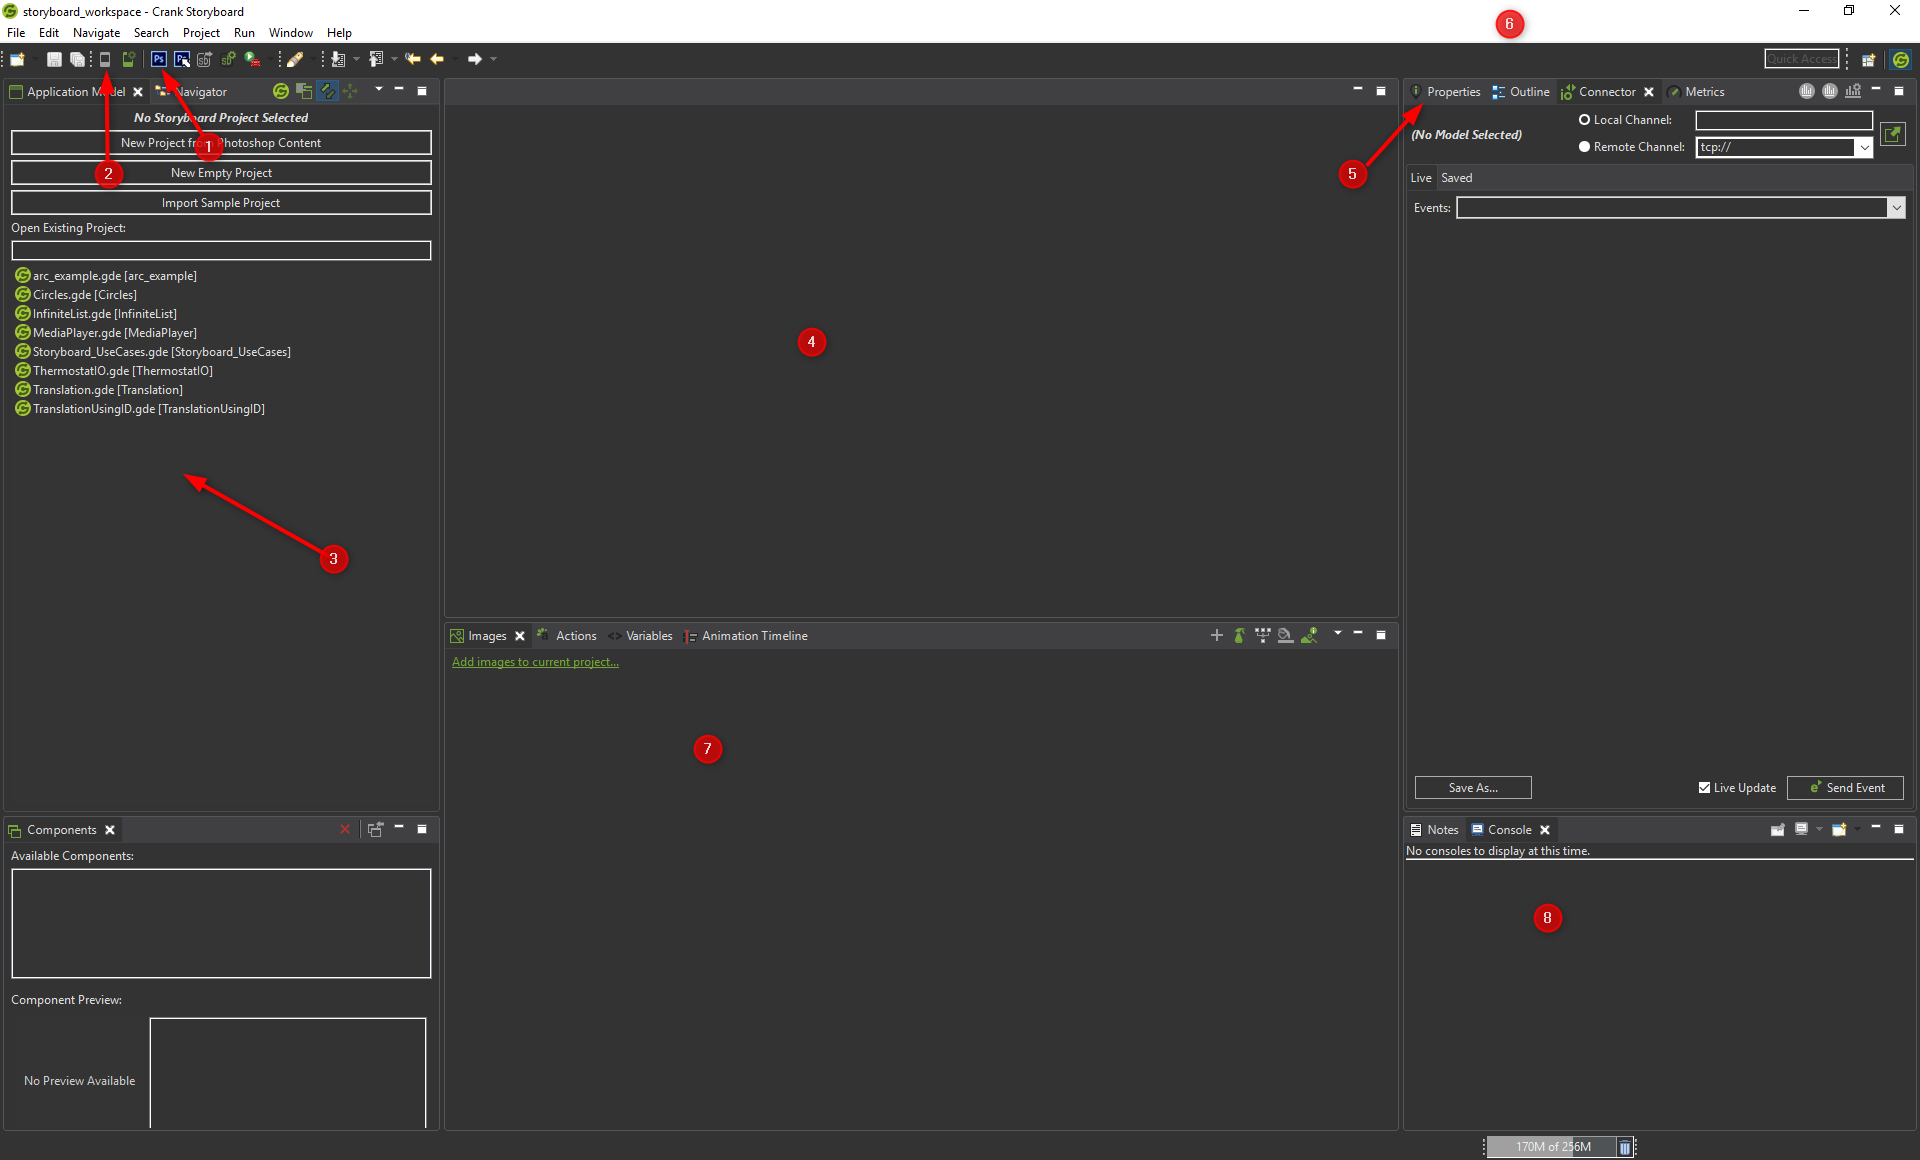
\includegraphics[width=\textwidth]{img/3_entwicklung_neues_kontept/2020-06-15_10h33_25}
%	\caption[Storyboard Start]{Storyboard Programm direkt nach dem Öffnen. 1: Photoshop-Import, 2: Simulation des Programms, 3: Auswahl der Bestehenden Projekte, 4: Editor, 5: Eigenschaften-Fenster, 6: Connector, 7: Bilder, Variablen, Actions, Timeline, 8: Konsolenausgabe}
%	\label{fig:storyboard_start}
%\end{figure}

%In Abbildung \ref{fig:storyboard_start} ist die grundsätzliche Aufmachung von Storyboard zu sehen. Von diesem Screen aus, können neue Projekte gestartet werden oder bestehende Projekte geöffnet werden.\\

%Das obere horizontale Menüband bietet die selben Funktionen wie in vielen anderen Programmen auch, es lassen sich Projekte und Dateien öffnen, neue Projekte und Dateien anlegen und diverse andere Einstellungen vornehmen. Unter dem Punkt 1 in Abbildung \ref{fig:storyboard_start} ist der Photoshop Import, mit dessen Hilfe ganze PSD-Dateien importiert werden können. Näheres zum Photoshop Import weiter unten im Kapitel.\\ 

%Punkt 2 ist die Simulation des aktuellen Projekts. Während der Simulation können Animationen und verschiedene Kontrollflüsse getestet werden. Durch einen Klick auf das Symbol öffnet sich ein Fenster in der vorher definierten Größe mit der Szene die vorher erstellt wurde.\\

%Bevor überhaupt ein Projekt geöffnet wurde und PSD-Dateien importiert und Projekte simuliert werden können, kann ein bestehendes Projekt geöffnen werden. Punkt 3 bietet hierfür eine Übersicht aller zuletzt geöffneten Projekte.\\

%Sobald ein Projekt geöffnet wurde öffnet sich zeitgleich, unter Punkt 4, der Editor. In diesem Editor, findet sich die aktuelle Szene die bearbeiten werden kann.\\

%Um verschieden Elemente zu bearbeiten, gibt es die Möglichkeit ihre Eigenschaften, unter Punkt 5, einzusehen. Die Eigenschaften enthalten unter anderem allgemeine Größen wie, die Position, die Größe und den Alpha-Wert. Außerdem gibt es noch Größen die sich nur auf das aktuelle Element beziehen, z.B. bei einer Text Render Extension, welcher Text in welcher Farbe und welcher Schriftgröße angezeigt werden soll.\\

%Unter Punkt 6 findet sich der Connector. Mit dem Connector lassen sich verschiedene Eingangssignale simulieren. Mit einem Schieberegler kann beispielsweise die Geschwindigkeit verändert werden. Im Hintegrund reagiert ein LUA-Skript auf dieses Signal und verändert die Eigenschaften eines gezeichneten Elements.\\

%Importierte Bilder, erstellte Variable, Aktionen und Animationen finden sich bei Punkt 7. Von dort können importierte Bilder in den Editor gezogen werden und angepasst werden. Variablen die unter Controls erstellt wurden können hier eingesehen und verwaltet werden. Aktionen wie ein Mausklick auf ein Element oder das Starten der Applikation können hier empfangen werden und verschiedene Reaktionen ausgelöst werden. In der Animation Timeline können Eigenschaften von Controls animiert werden.\\

%Um zu debuggen gibt es die Möglichkeit Text durch die LUA-Skripte auszugeben, diese werden unter Punkt 8 angezeigt. Ebenfalls werden dort Fehlermeldung und diverse andere Meldungen ausgegeben.\\

\subsubsection{Photoshop Import}

Nach dem Erstellen eines neuen Projekts, gibt es die Möglichkeit direkt eine Photoshop-Datei zu importieren. Dieser Prozess erspart das einzelne Hinzufügen und Platzieren von grafischen Elementen im Editor. %die Zeit spart.

\begin{figure}[htb]
	\centering
	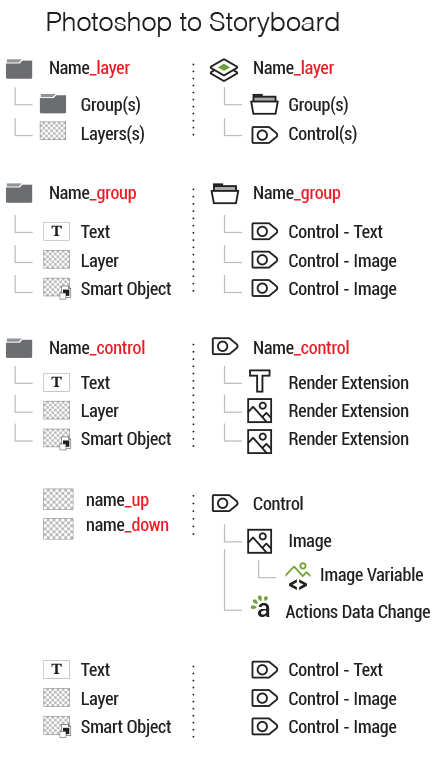
\includegraphics[width=8cm]{img/3_entwicklung_neues_kontept/story_psd}
	\caption[Hierarchie Modell für den Import von Photoshop-Dateien in Storyboard]{Hierarchie Modell für den Import von Photoshop-Dateien in Storyboard \cite{storyboard_doku_psd}}
	\label{fig:story_psd}
\end{figure}

Die Grafiken werden in bestimmten Ebenen gruppiert und nach einem Schema benannt. In Abbildung \ref{fig:story_psd} ist die Hierarchie zu sehen. Auf der linken Seite sind die Photoshop relevanten Elemente abgebildet, rechts daneben die Storyboard betreffenden.\\

Ein Ordner der in Photoshop mit \glqq \_layer\grqq{} endet wird auch als Layer in Storyboard eingefügt. Unterhalb dieses Layers, kann eine weitere Gruppierung existieren, sowie eine oder mehrere Photoshop-Ebenen.\\

Die Endung \glqq \_group\grqq{} erstellt eine Gruppierung in Storyboard. Innerhalb der Gruppe können sich Ebenen, Textebenen, sowie Smart Objects befinden. Jede dieser Ebenen wird zu einem Control in Storyboard. Ein Control Objekt besteht in Storyboard aus Render Extensions. Render Extension können Text, Bilder, Kreisbögen und ähnliches sein.\\

Gruppierungen mit der Endung \glqq \_control\grqq{} fassen ein Control Objekt in Storyboard zusammen. Alle Ebenen darunter werden zu Render Extensions die zu dem Control Objekt gehören. Mit Render Extensions können Control Objects einfache bis komplexe Aufgaben erfüllen. Ein Control Object mit zwei Image Render Extensions kann z.B. einen Button im Normal- und Gedrückt-Zustand darstellen.\\

Ein Button kann ebenfalls aus Photoshop importiert werden. Dazu wird ein Photoshop-Layer mit \glqq name\_up\grqq{} und \glqq name\_down\grqq{} benötigt. Storyboard erstellt aus diesen zwei Layern, ein Control Object mit einer Image Render Extension. Das Ändern des Bildes wird hier mit einer \glqq Image Variable\grqq{} und einer Action realisiert. Die Action wird aktiviert sobald innerhalb des Buttons geklickt wird und ändert dann die Quelle für das Bild in der \glqq Image Variable\grqq{}. Einzelne Layer, mit oder ohne Text, werden in Control Objects mit entsprechender Render Extension umgewandelt.\\


Für den Import in Storyboard wurde eine Photoshop-Datei erstellt. Die Photoshop-Datei besteht aus zwei Nadelinstrumenten, wie es von den Use Cases aus den vorherigen Kapiteln gefordert ist. Jedes Nadelinstrument besteht aus einem Hintergrund, dem äußeren Kreisbogen mit Zahlen, der Nadel, dem inneren Ring und der digitalen Anzeige. In der Datei gibt es zusätzlich noch zwei ausgeblendete Layer \glqq Overlay\_Layer\grqq{} und \glqq Telltales\_Group\grqq{}. Damit bei einem Import nicht direkt alle Layer in den aktiven Bildschirm geladen werden, können verschieden Layer ausgeblendet werden. Ausgeblendete Layer werden als \glqq Unused Layer\grqq{} importiert und können später bei Bedarf eingefügt werden.\\

\begin{figure}[htb]
	\centering
	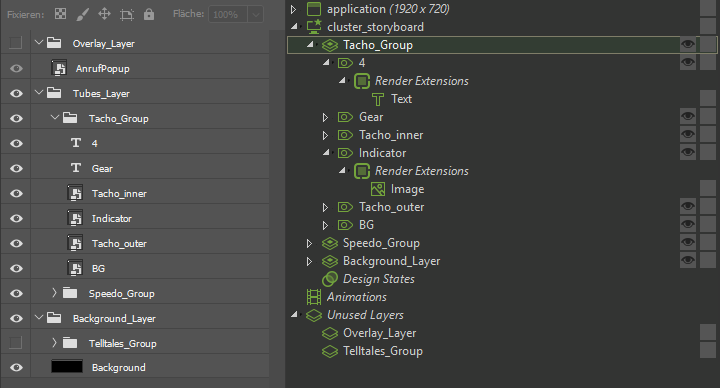
\includegraphics[width=\textwidth]{img/3_entwicklung_neues_kontept/vgl_psd_story}
	\caption[Vergleich Photoshop-Ebenen mit Storyboard-Ebenen]{Vergleich Photoshop-Ebenen (links) mit Storyboard-Ebenen (rechts)}
	\label{fig:vgl_layer}
\end{figure}

\newpage

In Abbildung \ref{fig:vgl_layer} ist die Aufteilung der Ebenen zu sehen. Links ist die Aufteilung in Photoshop zu sehen, rechts die Aufteilung in Storyboard direkt nach dem Import. In Photoshop wurden zwei Gruppen-Ordner angelegt unterhalb des \glqq Tube\_Layer\grqq{}. Zum einen die \glqq Tacho\_Group\grqq{} und zum anderen die \glqq Speed\_Group\grqq{}. Diese beiden Gruppen werden ebenfalls als Gruppierung in Storyboard eingefügt. Als Beispiel wird die \glqq Tacho\_Group\grqq{} genommen. Unterhalb der Gruppe in Photoshop, sind zwei Text-Ebenen und vier Ebenen mit Grafiken. In Storyboard werden diese Ebenen als Control mit den entsprechenden Render Extension eingefügt. Die Ebene \glqq 4\grqq{} ist in Photoshop eine Text-Ebene und wird in Storyboard als Control mit einer Text Render Extension eingefügt. Das selbe gilt für die Grafiken z.B. in Layer \glqq Tacho\_inner\grqq{} ist in Photoshop eine Ebene mit Grafik, in Storyboard wird hierfür ein Control mit einer Image Render Extension erstellt.

\subsubsection{Cluster HMI}

Der erste Use Case beschäftigt sich vor allem mit Nadelinstrumenten. In diesem Unterkapitel wird darauf eingegangen wie ein Nadelinstrument in Storyboard umgesetzt wird.\\

Ausgangspunkt ist ein Projekt direkt nach dem Import der Photoshop-Datei aus dem vorherigen Kapitel. Die zwei Nadelinstrumente aus der Photoshop-Datei werden korrekt in der Szene dargestellt. Zunächst muss die Größe des Controls mit der Nadelgrafik angepasst werden. Die Größe muss dem äußeren Ring aus Abbildung \ref{fig:img_prop_outer_tacho} entsprechen. Der äußere Ring ist ein Kreisbogen. Das Control-Element besitzt eine Breite von 548 Pixeln, was dem Durchmesser entspricht. Aufgrund der Abschrägung auf der Unterseite ergibt sich eine Höhe von 495 Pixeln. Das Control Object der Nadel muss die selbe Größe haben damit sich der Rotationspunkt an der richtigen Position befindet.\\

\begin{figure}[htb]
	\centering
	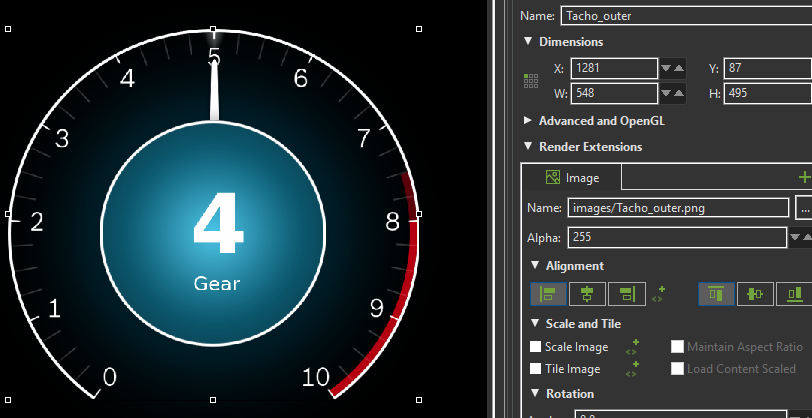
\includegraphics[width=\textwidth]{img/4_hmi_tools/anpassung_indicator}
	\caption{Grafik und Eigenschaften des äußeren Rings des Tachos}
	\label{fig:img_prop_outer_tacho}
\end{figure}

Innerhalb des Control-Elements muss die Grafik um 261 Pixel nach rechts verschoben werden, da die Grafik eine Breite von 26 Pixeln besitzt. Ansonsten würde die Nadel in der oberen linken Ecke dargestellt werden und nicht mittig. Anschließend müssen nur noch die Einstellungen für die Rotation vorgenommen werden. Das Rotationszentrum muss auf die Mitte des Control-Elements gelegt werden. \glqq Rotate around center of control\grqq{} führt nicht zum gewünschten Ergebnis. Für eine korrekte Rotation muss der X- und Y-Wert jeweils auf 274 gesetzt werden, die Hälfte von 548. Wird der Winkel jetzt verändert, rotiert die Nadel direkt am äußeren Ring entlang.\\

Damit während der Simulation die Nadel bewegt werden kann, muss mit Events und LUA-Skripten gearbeitet werden. Mit den LUA-Skripten können komplexe Funktionen umgesetzt werden. LUA kann auf alle Eigenschaften der Render Extensions zugreifen und sie ändern.\\

Zunächst muss ein Event erstellt werden. Events können bei verschiedenen Ereignissen ausgelöst werden um benutzerdefinierte Funktionen ( z.B. in LUA) auszuführen. Das Event \glqq cluster\_update\grqq{} ermöglicht, dass während der Simulation verschiedene Werte veränderbar sind.\\

\begin{figure}[htb]
	\centering
	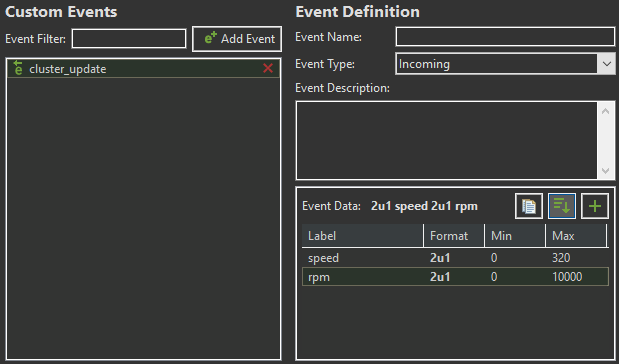
\includegraphics[width=\textwidth]{img/4_hmi_tools/event_indi_story}
	\caption{Cluster Update in Event Storyboard}
	\label{fig:event_story}
\end{figure}

Jeder Wert der änderbar sein soll, muss im Event als Label angelegt werden. Ein Label besteht aus einem Namen, Datentyp, minimalem Wert und maximalem Wert. In Abbildung \ref{fig:event_story} ist ein beispielhaftes Event mit Labeln abgebildet. Das Event ist über den Storyboard Connector erreichbar. Dort kann das Event ausgewählt und die Werte können über Schieberegler verändert werden.\\

In der callbacks.lua wird eine Funktion erstellt, welche ebenfalls \glqq cluster\_update\grqq{} heißt. Um eine bessere Übersichtlichkeit zu gewährleisten werden das Event und die dazugehörige Funktion gleich benannt. Die callbacks.lua ist die Hauptskript-Datei, in der alle Funktionen implementiert werden die nötig sind. \\

\newpage

\lstset{language=[5.0]Lua}
\begin{lstlisting}[frame=htrbl, caption={callbacks.lua}, label={lst:callbacks_story}]
function cluster_update(mapargs)
--get all label values 
local speed = mapargs.context_event_data.speed
local rpm = mapargs.context_event_data.rpm
local speed_rot = interpolation(speed,0,320,-144,144)
local rpm_rot = interpolation(rpm,0,10000,-144,144)

--set all variables
gre.set_value("Speedo_Group.speedo_indicator.rotation", speed_rot)
gre.set_value("Tacho_Group.Indicator.rotation", rpm_rot)
end

function interpolation(x,x1,x2,y1,y2)
return y1+(y2-y1)/(x2-x1)*(x-x1)
end
\end{lstlisting}

Die \glqq cluster\_update\grqq{} Funktion, in Listing \ref{lst:callbacks_story}, muss alle Änderungen an den Werten einlesen und verarbeiten. Für das Nadelinstrument muss die Geschwindigkeit eingelesen und in einen Winkel umgerechnet werden. Mit \glqq mapargs.context\_event\_data.speed\grqq{} bzw. \glqq mapargs.context\_event\_data.rpm\grqq{} kann auf die Werte der Labels aus dem cluster\_update zugegriffen werden. Eine selbstgeschriebene Interpolationsfunktion berechnet aus der Geschwindigkeit einen Winkel für die Nadel. Anschließend wird mit der Funktion \glqq gre.set\_value()\grqq{} der berechnete Winkel an eine Variable ausgegeben.\\

Mit Hilfe einer Variablen können Eigenschaftswerte eines Control Objects zur Laufzeit verändert werden. Eine Variable kann über einen Rechtsklick auf ein Control Object erstellt werden. In dem sich öffnenden Fenster kann der Datentyp und der Name der Variable gewählt werden. Für die Nadelrotation wird eine Float Variable mit dem Namen \textit{rotation} erstellt. Im Eigenschaftsfenster des Control Objects muss die Variable mittels Databinding an die Eigenschaft \textit{Angle} gebunden werden. Das führt dazu, dass der Wert der Variable automatisch an die Eigenschaft weitergegeben wird.\\

Zum Schluss muss noch eine Action erstellt werden. Eine Action verbindet ein Event mit bestimmten Funktionen. In diesem Fall soll die LUA-Funktion \glqq cluster\_update\grqq{} ausgeführt werden, wenn das dazugehörige \glqq cluster\_update\grqq{} Event ausgelöst wird.\\

In der Mitte des linken Nadelinstruments muss die Geschwindigkeit zusätzlich digital angezeigt werden. Dazu muss zunächst ein Control Object mit einer Text Render Extension angelegt und korrekt positioniert werden. Mit der Text Render Extension lässt sich beliebiger Text anzeigen.\\

Das Control Object benötigt wieder eine Variable, dieses mal vom Datentyp String. Analog zur Nadelrotation, muss der Wert nun wieder in der \glqq cluster\_update\grqq{} Funktion eingelesen und in die Variable geschrieben werden. Über Databinding wird der Wert der Variable an die Eigenschaft \textit{Text} weitergegeben.\\

%bis hierhin neu

Unterhalb der digitalen Geschwindigkeit muss die dazugehörige Einheit angezeigt werden. Zusätzlich soll die Einheit umschaltbar zwischen Meilen und Kilometern pro Stunde sein.\\

Dem Control Object der digitalen Geschwindigkeit wird dazu eine weitere Text Render Extension hinzugefügt. Wie auch bei der Geschwindigkeitsanzeige muss auch hier eine Variable erstellt und die Verarbeitung in LUA programmiert werden. Allerdings muss dieses mal ein neues Label im \glqq cluster\_update\grqq{} Event angelegt werden. Für ein Umschalten zwischen zwei Zuständen, ist eine boolesche Variable ausreichend.\\

Als letztes wird noch ein Nachleuchten-Effekt benötigt. Der Nachleuchten-Effekt soll die Bewegung der Nadel verdeutlichen. Die für diesen Effekt erstellte Grafik, reicht von 0 bis 160 \si[per-mode=symbol]{\kilo\meter\per\hour} und nimmt damit genau die Hälfte des Nadelinstruments ein. Da sich die Geschwindigkeit stetig verändert, bewegt sich auch die Nadel. Bewegt sich die Nadel im Bereich unterhalb der 160 \si[per-mode=symbol]{\kilo\meter\per\hour} muss ein Teil der Grafik ausgeblendet werden. Also der Teil der von der Nadel bis zu 160 \si[per-mode=symbol]{\kilo\meter\per\hour} reicht. Bewegt sich die Nadel allerdings im Bereich oberhalb der 160 \si[per-mode=symbol]{\kilo\meter\per\hour} muss die komplette Grafik mit der Nadel rotieren.\\

Eine Maske wäre für diesen Effekt die beste Lösung. Durch eine Maskierung der Grafik, kann der nicht benötigte Teil ausgeblendet werden. Die Maske würde in diesem Fall aus einem Kreisbogen bestehen, der immer vom Anfang des Nadelinstruments bis zur Nadel reicht. Das Ende des Kreisbogens folgt also dynamisch der Nadel. Die Pixel der Grafik würden dann nur angezeigt werden wenn an dieser Stelle, auch ein Pixel in der Maske gesetzt ist.\\

Storyboard bietet allerdings keine Möglichkeit Masken zu benutzen. Auf Nachfrage beim Support wurde eine Lösung genannt die auf Shadern basiert. Die Anzahl an Shadern in eingebetteten System ist allerdings begrenzt. Das heißt, Shader sollten sparsam verwendet werden. Da es wichtigere Funktionen gibt als den Nachleuchten-Effekt, die zwingend Shader verwenden müssen, ist diese Lösung nicht nutzbar.\\

Zusammenfassend lässt sich sagen, dass sich die Use Cases aus diesem Kapitel leicht umsetzen lassen. Der Photoshop Import erleichtert das Einfügen von Elementen, da sie im voraus bereits in Photoshop platziert werden können. Somit lässt sich z.B. das Nadelinstrument innerhalb von wenigen Minuten einfügen. Allerdings ist die Erstellung der Funkionen in LUA außerordentlich aufwendig. Zudem ist es nicht möglich einen Nachleuchten-Effekt mittels Maskierung zu erstellen. Das führt dazu das Storyboard in der späteren Auswahl nicht berücksichtigt werden kann.\\

\subsubsection{Visual Appearance}
In diesem Kapitel geht es um die Darstellung der \ac{ACC}-Funktion. Der Zustand der \ac{ACC}-Funktion muss mit einem 3D-Modell eines Fahrzeugs dargestellt werden.\\

Ein 3D-Modell wird in Storyboard mit Hilfe der 3D-Model Render Extension umgesetzt. Sobald ein Control Object mit einer 3D Render Extension erstellt wird, öffnet sich ein Datei-Dialog (Abbildung \ref{fig:story_import}). In diesem Dialog kann ein bereits importiertes 3D-Modell ausgewählt oder eine neues importiert werden.\\

\begin{figure}[htb]
	\centering
	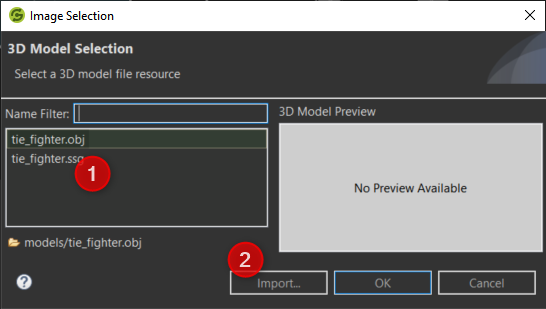
\includegraphics[width=12cm]{img/4_hmi_tools/model_import_story}
	\caption[3D-Modell Import Dialog in Storyboard]{3D-Modell Import Dialog 1:importierte Modelle, 2:Import Button für neue Modelle}
	\label{fig:story_import}
\end{figure}


Eine 3D-Szene besteht aus einem 3D-Objekt, einer Kamera und einem Licht. Die Kamera ist in dem Fall immer die Szene auf der gerendert wird. Das Licht sorgt dafür, dass realistische Schatten auf das 3D-Objekt fallen. Die 3D-Modell Render Extension besitzt eine größere Menge von Einstellungen, die in Abbildung \ref{fig:3d_model_story} dargestellt sind. Im Folgenden wird nur auf die wichtigsten Eigenschaften eingegangen.\\

\begin{figure}[htb]
	\centering
	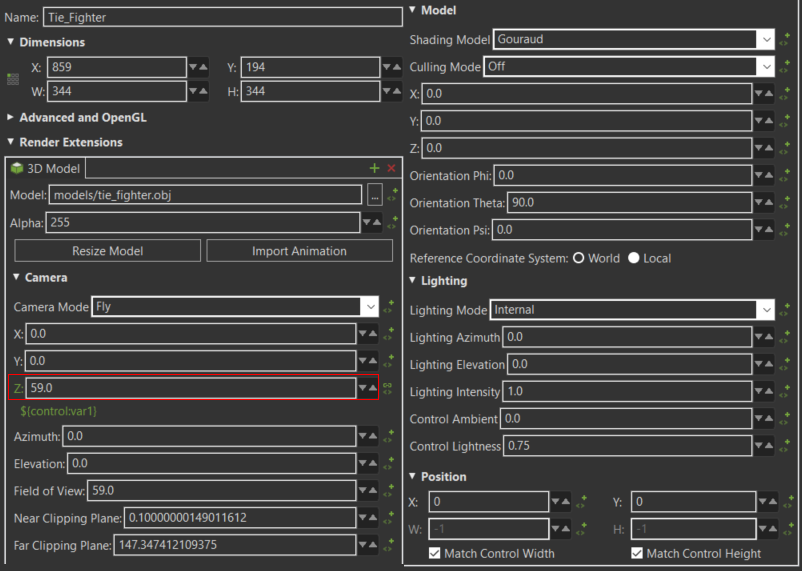
\includegraphics[width=\textwidth]{img/4_hmi_tools/3d_model_props}
	\caption[Einstellungen eines 3D-Models in Storyboard]{Einstellungen eines 3D-Models}
	\label{fig:3d_model_story}
\end{figure}

\newpage

Das 3D-Modell muss sich abhängig von der Geschwindigkeit nach vorne oder nach hinten bewegen. Diese Anforderung lässt sich in drei verschiedenen Varianten umsetzten. Zum einen kann die Eigenschaft Field of View verändert werden. Diese Eigenschaft verändert das Sichtfeld der Kamera. Ein höhere Wert sorgt dafür, dass das Modell kleiner wird. Ein kleinerer Wert lässt das Modell größer werden. Zum anderen kann die Kamera oder das Objekt über die Koordinaten bewegt werden.\\

Für die Umsetzung des Use Cases wird die Kamera in Z-Richtung bewegt. Die restliche Vorgehensweise ist analog zu den vorherigen Beispielen. Es wird wieder eine Variable benötigt und in LUA muss eine Verarbeitung der Werte stattfinden.

\subsubsection{Text- und Listenverhalten}
Im Use Case Text- und Listenverhalten muss eine scrollbare Liste umgesetzt werden. Die Liste sollte ca. 500 Einträge enthalten.\\

Um eine Liste in Storyboard zu erstellen, wird eine Tabelle benötigt. Zur Laufzeit kann diese Tabelle dynamisch mit Daten gefüllt werden. Zunächst muss eine Tabelle mit einer Spalte und einer Zeile erstellt werden. Die Tabelle wird später in LUA an die Anzahl der Einträge angepasst. Damit die Einträge dynamisch verändert werden können, wird eine Tabellen Variable benötigt. In diese Variable wird der Inhalt geschrieben, über Databinding werden die Daten an die Tabelle weitergegeben.\\

\lstset{language=[5.0]Lua}
\begin{lstlisting}[frame=htrbl, caption={callbacks.lua}, label={lst:callbacks_story}]
function CBInitTable()

-- read data
local file = assert(loadfile(gre.SCRIPT_ROOT .. "/words/wordList.txt"))
local words = file()

-- set table to 500 entries
gre.set_table_attrs("ListBehaviour.Playlist", {rows = 500})

-- save data in temp var
local data = {}
for row=1,500 do
data[string.format("ListBehaviour.Playlist.name.%d.1", row)] = words[row]

end

-- write data to variable
gre.set_data(data)
end
\end{lstlisting}

Als Quelle dient eine Textdatei, in dieser Datei sind alle Einträge enthalten. Damit die Liste zum Programmstart gefüllt wird, muss die Funktion aus Listing \ref{lst:callbacks_story} über eine Action ausgeführt werden. Die Funktion \textit{CBInitTable} liest die Einträge aus der \textit{wordList.txt} aus und schreibt sie in die Tabellen Variable.\\

In den Eigenschaften der Tabelle lässt sich noch einstellen wie gescrollt wird. Zur Auswahl steht einmal, von Eintrag zu Eintrag, oder pixelbasiert.\\

\subsubsection{Externe Daten}
Im Use Case Externe Daten soll überprüft werden, ob es möglich ist ein Video aus externer Quelle abzuspielen (z.B. Navigationsbild, Rückfahrkamera). \\

Damit ein Video in Storyboard abgespielt werden kann, wird ein Control Object mit der External Buffer Render Extension benötigt. In diesem Buffer können verschiedene externe Inhalte gerendert werden (z.B. Webbrowser oder Videos).\\

Um den Buffer mit einem Video zu befüllen, muss die Funktion \textit{gra.media.new.video} ausgeführt werden. Die Funktion wird von Storyboard bereitgestellt und wird nur über die Eigenschaften im Eigenschaftsfenster spezifiziert. In den Eigenschaften wird der Channel Name, die Video Quelle, sowie der External Buffer festgelegt. Der Channel Name ist wichtig, falls mit einer anderen Funktion das Video z.B. pausiert werden soll. In beiden Funktionen muss dann der gleiche Name stehen. Die Eigenschaft External Buffer Name stellt die Verbindung zum vorher erstellten External Buffer her.\\

Damit die Funktion \textit{gra.media.new.video} ausgeführt wird, wird ein Event benötigt. Dazu wird das Event \textit{MediaPlay} angelegt. Das Event kann z.B. über einen Klick auf einen Button ausgelöst werden und das Video wird abgespielt. Damit das Video gestoppt werden kann, wird noch das Event \textit{MediaStop} angelegt. Dieses Event löst die Funktion \textit{gra.media.stop} aus.\\

In diesem Fall soll das Video über den Storyboard Connector gestartet und gestoppt werden. Im \textit{cluster\_update} Event wird dazu ein neues Label erstellt. Das Label ist eine boolesche Variable. Mit diesen zwei Zuständen werden die zwei Events, \textit{MediaPlay} und \textit{MediaStop} ausgelöst. Bei dem booleschen Wert false wird das Video gestoppt und bei true wird das Video abgespielt.\\

Das Auslösen der Events erfolgt in der \textit{cluster\_update} Funktion. In Listing \ref{lst:media_story} ist der Code zu sehen. Zunächst wird der aktuelle Wert des Labels ausgelesen, anschließend wird je nach Zustand ein Event ausgelöst.\\

\begin{lstlisting}[frame=htrbl, caption={callbacks.lua}, label={lst:media_story}]
local play = mapargs.context_event_data.playVideo
if play == 1 then
	gre.send_event("MediaPlay")
	playerAttr["hidden"] = 0
	gre.set_control_attrs("VideoPlayback",playerAttr)
else
	gre.send_event("MediaStop")
	playerAttr["hidden"] = 1
	gre.set_control_attrs("VideoPlayback",playerAttr)
end
\end{lstlisting}

Abschließend lässt sich sagen, dass sich mit Storyboard der Großteil der Use Cases umsetzen lässt. Einzig der Nachleuchten-Effekt ist nicht umsetzbar. Der grafische Teil der Use Cases ist meist schnell realisiert, allerdings ist das Erstellen der einzelnen Funktionen dahinter mühselig. Oft muss für eine einfache Funktion ein Event, eine Action und eine LUA-Funktion erstellt werden, auch für relativ triviale Funktionen. Das sorgt in größeren Projekten für eine schlechte Übersichtlichkeit, zudem erschwert das die Modifizierbarkeit. Muss eine Funktion geändert werden, muss eventuell das Event, die Action und die LUA-Funktion verändert werden. Qt bietet dazu mit dem Qt Design Studio einen Kontrast und wird deshalb im nächsten Kapitel evaluiert.\\

\subsection{Qt}
\label{qt}
Qt wurde das erste mal 1995 von der Firma Trolltech veröffentlicht. Qt war damals noch ein Framework und keine komplette Entwicklungsumgebung. Entwickelt wurde dieses Framework von zwei norwegischen Entwickeln, Haavard Nord und Eirik Chambe-Eng. Heute besteht Qt aus einer umfangreichen Entwicklungsumgebung, dem QtCreator, sowie einem Design Tool, dem Qt Design Studio. \cite{qt_company}\\

Im Qt Design Studio werden die einzelnen grafischen Elemente zu einem \ac{HMI} zusammengefügt. Qt hat dafür eine eigene Skriptsprache entwickelt. \ac{QML} ist angelehnt an CSS und JSON und gehört zu den Auszeichnungssprachen (engl. Markup Language). Auszeichnungssprachen sind für die Gliederung und Formatierung von Text, Daten, etc. gedacht. Innerhalb von \ac{QML} kann zusätzlich die Javascript Syntax verwendet werden.\\

\subsubsection{Photoshop Import}

Als Verbindung zwischen Photoshop und Qt bietet Qt ein Plugin für Photoshop an. Die Photoshop Bridge wird als zxp-Datei geliefert und lässt sich über den ZXP Installer installieren. Das Photoshop Plugin wurde im Rahmen der Arbeit nicht evaluiert, daher wird nicht näher darauf eingegangen.\\


\subsubsection{Cluster HMI}
In diesem Use Case muss wieder ein Nadelinstrument umgesetzt werden.\\

Das Nadelinstrument wird mit der Image-Komponente zusammengestellt. Für jede Grafik des Nadelinstruments wird eine Image-Komponente im Qt Design Studio erstellt. Die Komponenten müssen in der Hierarchie anschließend in die richtige Reihenfolge gebracht werden, damit das Nadelinstrument korrekt dargestellt wird. Im Qt Design Studio steht die unterste Ebene in der Hierarchie an erster Stelle.\\

Um die Rotation der Nadel zu ermöglichen, wird die Item-Komponente benötigt. Ein Item kann als Container verstanden werden. In einem Item können sich mehrere Objekte befinden. Diese Objekte können dann z.B. im Koordinatensystem des Items positioniert werden. Im Fall der Nadel kann die Grafik an einer bestimmten Position um einen bestimmten Punkt rotieren. Das heißt Die Nadel wird im Koordinatensystem der Item-Komponente Positioniert und die Item-Komponente wird mittig im Nadelinstrument positioniert. Anschließend kann über die Eigenschaft \textit{rotation} die Nadel rotiert werden.\\

%nadelrotation fertig

In der Mitte des Nadelinstruments muss die Geschwindigkeit wieder digital angezeigt werden. Außerdem wird auch wieder die umschaltbare Einheit benötigt. Beide Funktionen sind mit der Text-Komponente umsetzbar. Über die Eigenschaft \textit{text} kann der angezeigte Text jederzeit verändert werden.\\

%digital fertig

Die Nadel soll einen Nachleuchten-Effekt besitzen. Qt bietet dafür die OpacityMask-Komponenten. Mit dieser Komponente lassen sich Grafiken einfach maskieren. In Abbildung \ref{fig:qt_mask} ist eine Übersicht zur Maske dargestellt.\\

\begin{figure}[htb]
	\centering
	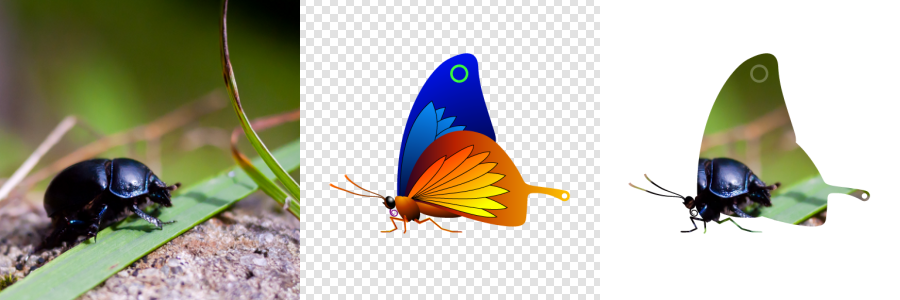
\includegraphics[width=\textwidth]{img/4_hmi_tools/qt_mask}
	\caption[Maskierung einer Grafik in Qt]{Maskierung einer Grafik. Links das Ursprungsbild, in der Mitte die Maskengrafik, rechts das maskierte Ursprungsbild. \cite{qt_mask}}
	\label{fig:qt_mask}
\end{figure} 

Die Maske besteht aus einem Ursprungsbild und der Maskengrafik. Ein Pixel im Ursprungsbild wird nur angezeigt, wenn in der Maskengrafik an der gleichen Position auch ein Pixel ist. Ist der Pixel an der gleichen Position nicht vorhanden, wird der Pixel des Ursprungsbildes ausgeblendet.\\

Mit dieser Komponente lässt sich der Nachleuchten-Effekt umsetzten. Das Ursprungsbild ist die Nachleuchten-Grafik und die Maskengrafik ist ein Kreisbogen (Arc). Der Kreisbogen wird mit der Arc-Komponente umgesetzt. Der Arc startet bei 0 \si[per-mode=symbol]{\kilo\meter\per\hour} und endet immer an der Nadel. Dadurch wird die Nachleuchten Grafik immer nur dort angezeigt, wo sie benötigt wird. Das mit rotieren der Grafik ab 160 \si[per-mode=symbol]{\kilo\meter\per\hour} ist entweder über eine Animation oder über eine Simulation mit Javascript umsetzbar.\\

Um die Bewegung der Nadel und den Nachleuchten-Effekt mit einer Animation zu lösen, wird zunächst eine neue Animation-Timeline erstellt. In der Animation-Timeline können für die verschiedenen Komponenten Keyframes festgelegt werden. Eine Animation besteht aus mehreren Frames. Ein Keyframe legt den Wert einer Eigenschaft in einem bestimmten Frame fest. Zwischen zwei Werten in unterschiedlichen Frames wird interpoliert. Für die Nadel wird im ersten Frame die Eigenschaft \textit{rotation} so festgelegt, dass 0 \si[per-mode=symbol]{\kilo\meter\per\hour} angezeigt werden. Anschließend wird ein Keyframe erstellt und die Rotation in der Timeline gespeichert. Danach muss die Nadel auf die Endposition, damit im letzten Frame erneut die Rotation mit einem Keyframe gespeichert werden kann. Beim Abspielen der Timeline bewegt sich die Nadel nun von 0 bis 320 \si[per-mode=symbol]{\kilo\meter\per\hour}. Das gleiche muss für die anderen Komponenten vorgenommen werden, damit auch der Nachleuchten-Effekt korrekt dargestellt wird.\\

Die Animation besteht insgesamt aus 320 Frames. Jeder Frame stellt damit genau 1 \si[per-mode=symbol]{\kilo\meter\per\hour} dar. Somit benötigt die QML-Datei später nur die Geschwindigkeit, da die Geschwindigkeit mit einem Frame der Animation gleichzusetzen ist. Zudem müssen keine Berechnungen in QML stattfinden.\\

%gefällt mir noch nicht
Für die Simulation im Qt Design Studio besteht die Möglichkeit mit Javascript ein Backend zu erstellen. Hierzu wird eine Javascript-Datei und eine QML-Datei erstellt. In der QML-Datei werden die benötigten Variablen und Timer programmiert. Ein Timer ruft in einem bestimmten Intervall eine Funktion aus der Javascript-Datei auf. In der Javascript Funktion wird dann ein Wert hoch- oder runtergezählt, z.B. die Geschwindigkeit. Der Wert wird in der QML zwischengespeichert und kann in einer anderen QML über Databinding an eine Eigenschaft übergeben werden.\\

%noch mehr dazu?
Der Use Case Cluster HMI erfordert ebenfalls die Implementierung von Warnlampen. Qt bietet dafür eine eigene Komponente, die IsoIcon-Komponente. IsoIcons können beliebig platziert werden. Ein Doppelklick auf das Element öffnet einen Auswahl-Dialog. In diesem Dialog sind alle Icons nach dem ISO Standard auswählbar. Über die Eigenschaften kann anschließend die Farbe konfiguriert werden.\\

\subsubsection{Visual Appearence}
Dieses Kapitel beschäftigt sich mit dem Anzeigen der \ac{ACC}-Funktion. Hierzu muss wieder ein 3D-Modell darstellbar sein. Qt bietet für 3D-Szenen QtQuick3D an. \\

Um 3D Modelle im FBX Format in QML zu nutzen, bietet Qt eine Import-Funktion an. Mit Hilfe der Import-Funktion wird aus dem 3D-Modell eine eigene QML-Datei erzeugt. Die QML-Datei wird später als benutzerdefinierte QML-Komponente benutzbar und kann dadurch in anderen QML-Dateien verwendet werden.\\

Im Qt Design Studio gibt es einen integrierten 3D-Editor. Es kann zwischen dem normalen Form-Editor und dem 3D-Editor gewechselt werden. Im Form-Editor werden die 2D QML-Komponenten dargestellt und können dort auch positioniert werden. Im 3D-Editor können alle 3D-Objekte wie z.B. Lichter, Modelle und Kameras positioniert, rotiert und skaliert werden. Im Form-Editor wird immer das aktuelle Kamerabild gerendert dargestellt. Abbildung \ref{fig:qt_3d} zeigt den 3D-Editor des Qt Design Studios.\\ 

\begin{figure}[htb]
	\centering
	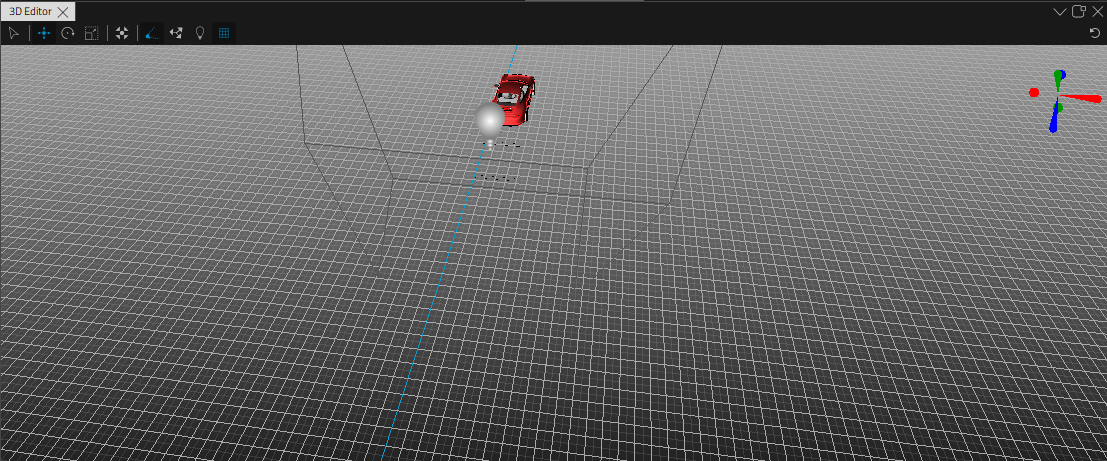
\includegraphics[width=\textwidth]{img/4_hmi_tools/3d_editor}
	\caption[3D-Editor in Qt]{Übersicht 3D-Editor im Qt Design Studio}
	\label{fig:qt_3d}
\end{figure}

Sobald alle Objekte in Position sind, muss noch die Y-Position des Autos als Alias exportiert werden. Ein Alias ermöglicht die Bearbeitung von internen Eigenschaften von außen. Die QML-Datei des 3D-Modells wird später in einer anderen QML-Datei verwendet. Ohne ein Alias wäre es nicht möglich auf die Y-Position des Fahrzeugs zuzugreifen. In der QML-Datei in der das 3D-Modell verwendet wird, lässt sich das Fahrzeug nach vorne oder hinten bewegen.\\

\begin{figure}[htb]
	\centering
	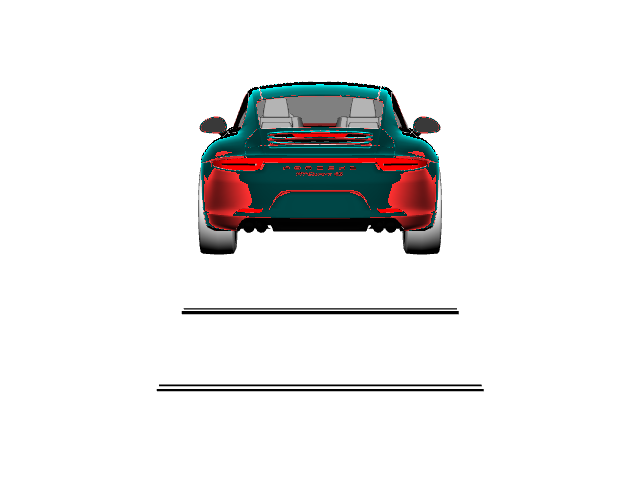
\includegraphics[width=\textwidth]{img/4_hmi_tools/qt_3d_render}
	\caption[Gerendertes Kamerabild einer 3D-Szene in Qt]{Das gerenderte Kamerabild als 3D-Szene in Qt}
	\label{fig:qt_render}
\end{figure}

Die fertige 3D-Szene ist in Abbildung \ref{fig:qt_render} zu sehen. Die Szene zeigt die Perspektive aus Sicht der Kamera. Die Szene ist im Form-Editor beliebig platzierbar.\\

\subsubsection{Text- und Listenverhalten}
%einleitender Satz

In Qt Design Studio werden Listen mit der Model/View Architektur erzeugt. Für die Liste wird dazu ein ListModel und eine ListView benötigt. Im ListModel werden die Daten hinterlegt und in der ListView angezeigt. Die Daten aus dem ListModel werden über ein Delegate an die ListView weitergegeben, ähnlich zum Beobachter-Muster. Diese vorgehensweise ist ähnlich zu dem \ac{MVC}-Muster.\\

%bild von https://doc.qt.io/qt-5/model-view-programming.html einfügen

Für die Evaluierung wird eine Liste mit dem XmlListModel erzeugt. Das XmlListModel bietet die Möglichkeit eine Liste in einer XML-Datei zu hinterlegen.\\

\newpage

\lstset{language=[5.0]Lua}
\begin{lstlisting}[frame=htrbl, caption={ListBehaviourModel.qml}, label={lst:list_qt}]
XmlListModel {
	id: xmlModel
	source: 																	"file:///C:/Users/plk4abt/Documents/instrumentCluster/backend/Data/listview_xml.xml"
	query: "/channel/item"

	XmlRole {
		name: "title"
		query: "title/string()"
	}
}
\end{lstlisting}

Listing \ref{lst:list_qt} veranschaulicht das Einbinden einer Xml-Datei. Die Daten sind damit im XmlListModel hinterlegt und können in einer ListView angezeigt werden. Die Daten aus dem XmlListModel werden über die Eigenschaft \textit{model} in die ListView geladen. Die Eigenschaft query in Zeile 4 gibt die Hierarchie in der XML-Datei vor. Das heißt jeder Listeneintrag muss zum einen innerhalb eines \textit{channel}-Tags liegen und zum anderen zwischen einem \textit{item}-Tag. In Zeile 7 wird festgelegt wo der Text für die Eigenschaft name hinterlegt ist. In diesem Fall liegt der Text zwischen dem \textit{title}-Tag. In Zeile 8 wird schließlich definiert, dass es sich um eine String-Variable handelt. Zum Vergleich ist in Listing \ref{lst:list_xml} ein Teil der XML-Datei abgebildet.\\

\lstset{language=[5.0]Lua}
\begin{lstlisting}[frame=htrbl, caption={list.xml}, label={lst:list_xml}]
<channel>
	<item>
		<title>A blog post</title>
	</item>
	<item>
		<title>Another blog post post</title>
	</item>
<\channel>
\end{lstlisting}


In der späteren Umsetzung wird auf ein eigenes Model zurückgegriffen. Dazu kann in C++ ein eigenes ListModel implementiert werden.\\ 

\subsubsection{Externe Daten}
Videos können im Qt Design Studio über die MediaPlayer-Komponente in die Video"=Output-Komponente geladen und abgespielt werden. In Listing \ref{lst:video_qt} ist der Code für den Videoplayer zu sehen.\\

\lstset{language=[5.0]Lua}
\begin{lstlisting}[frame=htrbl, caption={VideoPlayer.qml}, label={lst:video_qt}]
Item {
	width: Constants.width
	height: 720

	MediaPlayer {
		id: mediaplayer
		source: "file:///C:/Users/.../video/video.mp4"

	}

	VideoOutput {
		anchors.fill: parent
		source: mediaplayer

	}

	MouseArea {
		id: playArea
		anchors.fill: parent
		onPressed: mediaplayer.play();
	}
}
\end{lstlisting}

Die MediaPlayer-Komponente stellt die Quelldatei bereit, sowie Funktionen wie Play und Stop. Die Daten aus dem Video Player werden in den Buffer VideoOutput geladen, ähnlich wie in Storyboard. Die MouseArea-Komponente erlaubt das auslösen verschiedener Mausevents, z.B. einen Mausklick. Sobald innerhalb der MouseArea geklickt wird, wird mit \textit{mediaplayer.play()} das Video gestartet.\\

\subsection{Auswahl des HMI Tools}

Diese Kapitel beschäftigt sich mit der Auswahl des HMI Tools. Dafür werden alle Vor- und Nachteile aus den vorherigen Kapiteln gegenüber gestellt.\\

\subsubsection{Vor- und Nachteile CGI Studio}
CGI Studio wird schon mehrere Jahre bei Bosch verwendet. Durch die langjährige Nutzung, hat sich viel Fachwissen und Erfahrung im Umgang mit CGI Studio angesammelt. Bosch bestimmt zum Teil auch die Weiterentwicklung mit.\\

CGI Studio kann theoretisch alle benötigten Use Cases abdecken. Die Use Cases aus Kapitel \ref{use_cases} wurden aus CGI Studio abgeleitet. Doch wie in Kapitel \ref{cgi} beschrieben, gestaltete sich die praktische Umsetzung schwieriger als gedacht. Die Möglichkeit Widgets durch verschiedene DLL-Dateien zu laden, bietet Flexibilität, zeigt aber auch wie schnell das unübersichtlich wird. Vor dem Start, muss erst eine passende DLL-Datei gefunden werden und je mehr Projekte existieren, desto schwiergier wird die Suche.\\


\subsubsection{Vor- und Nachteile Storyboard}
Storyboard ist ein sehr einfach zu erlernendes Tool. Die Entwicklungsumgebung ist sehr übersichtlich. Da nur relativ wenige Render Extension zur Auswahl stehen, sind die Funktionen sehr begrenzt. Diese Begrenzung verringert aber gleichzeitig die Komplexität. Mit Hilfe von LUA lassen sich jedoch komplexere Funktionen umsetzen. Storyboard konnte nahezu alle Use Cases erfüllen. Die meisten Informationen sind in der ausführlichen Dokumentation zu finden, falls etwas nicht in der Dokumentation auffindbar ist, hilft der kommerzielle Support schnell weiter. \\

Bei manchen Use Cases gab es kleiner Probleme mit der Umsetzung. So ist das Erstellen von Übersetzungen unnötig kompliziert. Im Tool gibt es bereits eine Übersicht der Übersetzungen, jedoch können diese dort nicht bearbeitet werden. Stattdessen muss die CSV-Datei geöffnet und bearbeitet werden. Der größte Nachteil ist allerdings, dass der Nachleuchten Use Case nicht umgesetzt werden kann. Storyboard hat im Nachgang noch eine mögliche Lösung geliefert, allerdings basiert diese auf Shadern. Da die Anzahl der Shader begrenzt ist und für wichtigere Funktionen benötigt wird, ist diese Lösung nicht nutzbar. \\

Die Use Cases haben gezeigt, dass es möglich ist die View in Storyboard umzusetzen. Allerdings ist nicht ersichtlich wie der Rest der Architektur (Controller und Model) umzusetzen sind. Es existiert die Möglichkeit, Events als C bzw. C++ Header zu exportieren. Dadurch soll der Zugriff auf Events von außerhalb der Storyboard Anwendung möglich sein.\\
 %quelle http://resources.cranksoftware.com/cranksoftware/v6.0.0/docs/webhelp/ch07s03.html\\

\newpage
Damit wäre es theoretisch möglich die Architektur umzusetzen, allerdings müssten das Model und der Controller außerhalb von Storyboard implementiert werden.\\
 

\subsubsection{Vor- und Nachteile Qt}
%Qt besteht eigentlich nur aus dem Qt Creator. Innerhalb des Qt Creator gibt es noch das Design Studio und den Qt Designer. Beide Tools existieren ebenfalls als eigenständige Version. Wie im Kapitel \ref{qt} erläutert, wurden die Use Cases komplett im Design Studio umgesetzt. Die spätere Implementierung erfolgt allerdings im Qt Creator.\\

Ein großer Vorteil von Qt ist die Opensource Variante und die dadurch existierende Support Community. Durch die große Anzahl an Nutzern, werden Bugs schneller gefunden. In den vorhandenen Foren gibt es zudem eine Vielzahl von Fragen und Antworten rund um das Qt Framework. Kann eine Frage dadurch nicht beantwortet werden, bietet Qt noch einen kommerziellen Support. Das Qt-Framework beinhaltet von Haus aus sehr viele Funktionen, das spart Entwicklungsaufwand. Trotzdem können eigene Funktionen durch die Auszeichnungssprache QML entwickelt werden. Die Funktionen lassen sich später in jedem Projekt wiederverwenden, dadurch reduziert sich ebenfalls der Entwicklungsaufwand. Mit dem QtCreator stellt Qt zudem eine All-in-one Lösung bereit. Im QtCreator ist bereits das Qt Design Studio integriert. Dadurch können die Designer die \ac{HMI} im Qt Design Studio entwerfen und später die \ac{HMI} zum QtCreator Projekt hinzufügen.\\

Der große Funktionsumfang ist zeitgleich auch ein Nachteil. Vor allem am Anfang erschlägt Qt mit seiner Vielfalt. Das erhöht die Einarbeitungszeit im Vergleich zu Storyboard, liegt aber weiterhin deutlich unter der Einarbeitungszeit die für CGI Studio notwendig ist.\\

In Qt Design Studio lässt sich die View problemlos umsetzen. In Verbindung mit dem QtCreator, lassen sich ebenfalls das Model und der Controller implementieren.\\

\subsubsection{Auswahl des HMI Frameworks}

In Tabelle \ref{tab:tools} sind alle Vor- und Nachteile der einzelnen Frameworks zusammengefasst. Mit Hilfe dieser Übersicht muss ein \ac{HMI} Framework ausgewählt werden.\\

Storyboard kann bei der Auswahl nicht berücksichtigt werden, da ein must-have Use Case nicht erüllt werden kann. Die Auswahl muss also zwischen CGI Studio und Qt getroffen werden. Bei einem Vergleich der Vor- und Nachteile von Qt und CGI Studio gewinnt Qt. Während der Benutzung von Qt haben sich kaum Nachteile gezeigt. In Qt konnten alle wichtigen Use Cases zufriedenstellend umgesetzt werden. Nach einer kurzen Einarbeitungszeit funktioniert das Arbeiten in Qt flüssig. Auftretende Probleme konnten meist durch eine kurze Internetrecherche gelöst werden. Das Lösen der Probleme durch Internetrecherche ist der großen Community zu verdanken. Qt hat sehr viele Nutzer, dadurch werden auch viele Probleme gefunden und gelöst. Im Hinblick auf die ISO 25010 Kriterien, hilft das vor allem dem Punkt Reliability (Zuverlässigkeit). Dessen Unterpunkte in der Gewichtung zwischen 18 und 21 von 31 Punkten erreicht haben und damit zu den wichtigeren Punkten gehören.\\


Da die Use Cases von CGI Studio abgeleitet sind, kann CGI Studio alle Use Cases umsetzen. Die Probleme mit CGI Studio sorgen dafür, dass CGI Studio Qt unterliegt. Im Gegensatz zu Qt kann bei CGI Studio nicht im Internet recherchiert werden Es gibt einfach keine Nutzer außerhalb von Bosch, die im Internet nach Hilfe suchen. Bosch ist einer der Hauptnutzer und somit auch Tester von CGI Studio. Bugs und Fehler werden dadurch eventuell zu spät gefunden. Die Erfahrung hat gezeigt, dass es auch schwierig sein kann die richtige Person zu finden die, bei Problemen oder Fragen, helfen kann.\\



\begin{table}[h]
	\centering
	\caption[Übersicht der Vor- und Nachteile der einzelnen Frameworks]{Übersicht der Vor- und Nachteile der einzelnen Frameworks}
	\label{tab:tools}
	\begin{tabular}{|p{1.6cm}|p{4.3cm}|p{4.3cm}|p{4.3cm}|}
		\cline{2-4}
		\multicolumn{1}{c|}{}      & CGI Studio                                     & Storyboard                                  & Qt                                                  \\ \hline
		\multirow{15}{*}{Vorteile} & aktuelles Standard-Tool                        & schnelle Einarbeitung                       & All-in-one Lösung durch QtCreator                   \\ \cline{2-4}
		                           & viel Expertise innerhalb von Bosch             & ausführliche Dokumentation                  & ausführliche Dokumentation                          \\ \cline{2-4}
		                           & besitzt alle nötigen Funktionen                & simpler Photoshop Import                    & eigenes Photoshop Plugin                            \\ \cline{2-4}
		                           & Bosch bestimmt Weiterentwicklung mit           &                                             & große Anzahl an vorgefertigten Funktionen           \\ \cline{2-4}
		                           &                                                &                                             & Möglichkeit zur Entwicklung eigener Funktionen      \\ \cline{2-4}
		                           &                                                &                                             & Möglichkeit zur Wiederverwendung eigener Funktionen \\ \hline
		\multirow{9}{*}{Nachteile} & Kaum Support von außen möglich                 & hoher Implementierungsaufwand in LUA        & etwas längere Einarbeitungszeit nötig               \\ \cline{2-4}
		                           & Wissen konzentriert sich auf Projektbeteiligte & Übersetzungen hinzufügen kompliziert        &                                                     \\ \cline{2-4}
		                           & Veraltete Widgets sind fehleranfällig          & keine Masken-Funktion (Ausschlusskriterium) &                                                     \\ \hline
	\end{tabular} 
	
\end{table} 



Im Hinblick auf das Architektur-Konzept und die Vor- und Nachteile ist Qt die beste Wahl.\\



% % !TEX root = Hauptdatei.tex
\section{Implementierung in QtCreator}\label{hauptabschnitt_2}

Diese Kapitel beschäftigt sich damit, wie eine \ac{HMI} in Qt im Hinblick auf das Architektur-Konzept umgesetzt werden kann.\\

\subsection{Simulation der Fahrzeugdaten}
Normalerweise erhält das \ac{HMI} die Daten des Fahrzeugs vom \ac{KSS} über \ac{CAN}. Für das Proof-of-Concept wird eine Simulation der Daten mit einem UI-Window von Qt realisiert. Qt ermöglicht mit dem Qt Designer die Entwicklung von Formsanwendungen. Die Formsanwendung soll als Dashboard dienen, in dem verschieden Daten zur Laufzeit manipuliert werden können (z.B. Geschwindigkeit, Drehzahl, etc.).\\

%quelle https://doc.qt.io/qt-5/designer-to-know.html
\begin{figure}[htb]
	\centering
	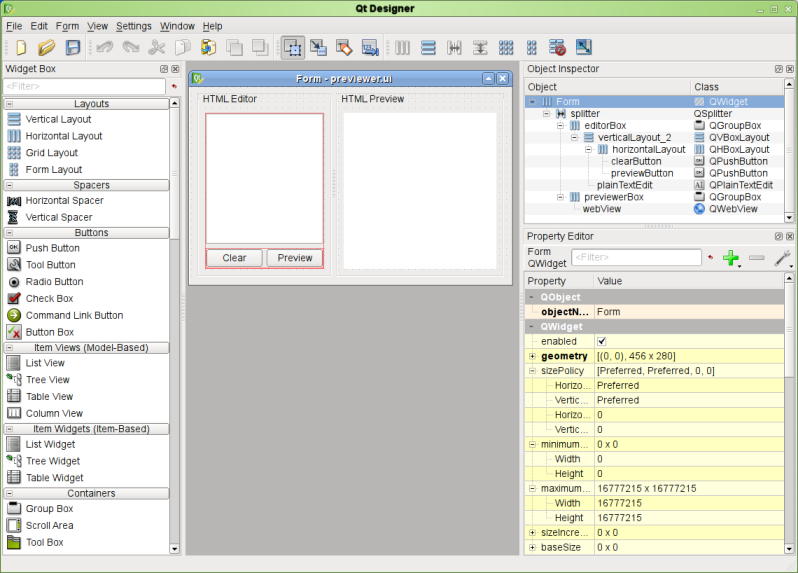
\includegraphics[width=\textwidth]{img/5_implementierung/qt_designer}
	\caption[Übersicht des QtDesigners]{Übersicht des QtDesigners \cite{qt_designer}}
	\label{fig:qt_designer}
\end{figure}

Abbildung \ref{fig:qt_designer} zeigt eine Übersicht des Qt Designer. Links ist eine Auswahl der verschiedenen Forms-Elemente zu sehen. Diese können per Drag and Drop in das Fenster in der Mitte gezogen werden. Qt erstellt für diese Fenster jeweils eine Header-Datei und Quell-Datei, diese Dateien ermöglichen das Einlesen und die Verarbeitung der Werte in C++.\\

Für das Proof-of-Concept wird ein Dashboard implementiert. Das Dashboard besteht aus verschiedenen Slidern, Combo Boxen, Buttons und anderen Formselementen. Abbildung \ref{fig:ui_window} zeigt eine Version dieses Fensters.\\

\begin{figure}[htb]
	\centering
	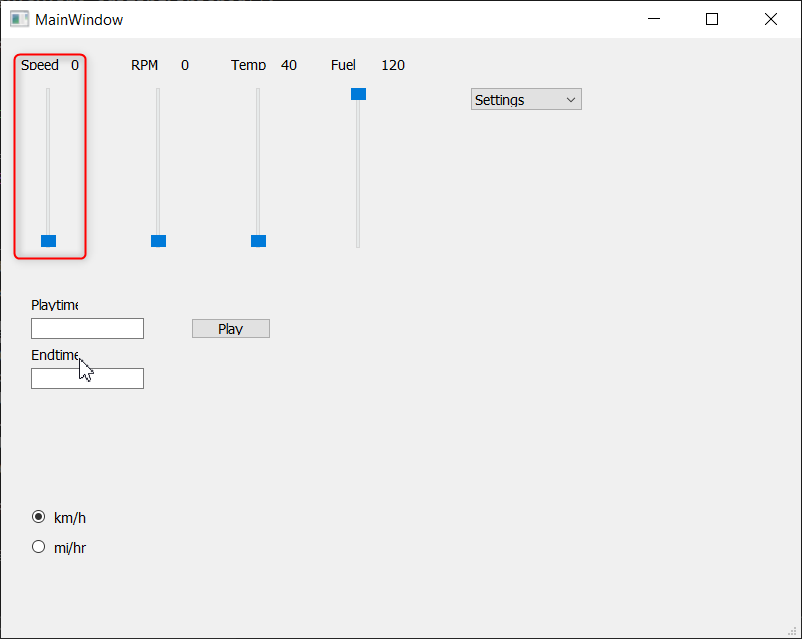
\includegraphics[width=\textwidth]{img/5_implementierung/ui_window}
	\caption[Aufbau des UI Formularfensters]{Aufbau des UI Formularfensters. Dieses ermöglicht im Folgenden die Eingabe der Fahrzeugdaten, welche im realen Fahrzeug vom Steuergerät gesendet werden.}
	\label{fig:ui_window}
\end{figure}

Jedes Formselement bietet verschiedene Funktionen um die Werte auszulesen. Der Wert eines Sliders kann z.B. über die Funktion \textit{on\_speedSlider\_valueChanged(int value)} ausgelesen werden. Diese Funktion wird aufgerufen, sobald sich der Wert des Sliders verändert. Der Parameter \textit{value} beinhaltet dabei den aktuellen Wert.\\

\subsection{Implementierung des Models}
Das Model wird als eigenständige Klasse umgesetzt. Wie im Architektur-Konzept beschrieben, besteht das Model aus mehreren, austauschbaren Klassen. So existiert beispielsweise jeweils für die Geschwindigkeits-, Drehzahl-, Temperatur- und Tankanzeige eine eigene Klasse. Diese Klassen werden im Model zusammengeführt. Das Model ist damit ein Fassadenmuster und bietet ein Interface zu den einzelnen Klassen.\\

\begin{figure}[htb]
	\centering
	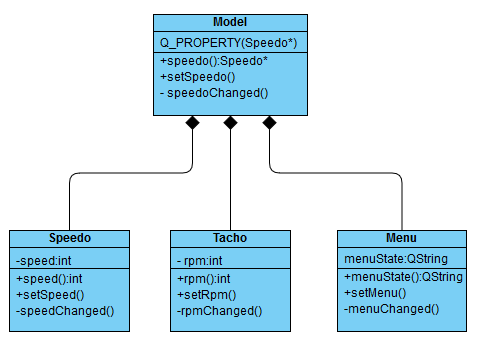
\includegraphics[width=10cm]{img/5_implementierung/implement_model}
	\caption[UML-Klassendiagramm des Models]{UML-Klassendiagramm des Models mit Beispiel-Modulen}
	\label{fig:implement_model}
\end{figure}

Abbildung \ref{fig:implement_model} zeigt ein beispielhaftes Klassendiagramm. Das Diagramm zeigt wie die Speedo-Klasse im Model implementiert ist und die Implementierung der Speedo-, Tacho- und Menu-Klasse. Die Speedo-Klasse ist für die Geschwindigkeit des Fahrzeugs verantwortlich. Jede weitere Klasse ist ähnlich aufgebaut, mit einer Set-, Get- und Signalfunktion. Mit der Set-Funktion wird mit Signals und Slots die Geschwindigkeit eingelesen. Die Signalfunktion zeigt an, ob der Wert geändert wurde. Bei einer Wertänderung kann der Wert dann mit der Get-Funktion ausgelesen werden.\\

Die Klassen innerhalb des Models werden über das Signals und Slots System von Qt mit Daten versorgt. Das Signals und Slots System entspricht der Umsetzung des Beobachter-Musters. Mit Signals und Slots können Daten klassenübergreifend ausgetauscht werden, ohne dabei die Klassen zu stark zu koppeln. Sobald ein Wert in der Formsanwendung verändert wird, wird ein Signal emittiert. Das Emittieren des Signals führt dazu, dass eine Set-Funktion in der Zielklasse ausgeführt wird. Dadurch ist der veränderte Wert in der Zielklasse verwendbar. Mit dieser Vorgehensweise werden alle Daten aus der Formsanwendung an die verschiedenen Klassen im Model verteilt.\\

Vom Model aus müssen die Daten in ähnlicher Form an den Controller bzw. die View verteilt werden. Bei der Verteilung an die View wird zusätzlich noch das Property System von Qt benötigt. Das Property System ermöglicht, dass die View die Daten aus dem Model auslesen und verarbeiten kann. %Property System genauer erklären?

Abbildung \ref{fig:uml_sequenz} zeigt ein UML-Sequenzdiagramm mit beispielhaften Signalen. Der Großteil der Daten kann direkt vom Model an die View gesendet werden. Das gilt für alle fahrzeugbezogenen Daten. Benutzereingaben werden hingegen zunächst vom Controller verarbeitet. Im Controller wird geprüft ob es notwendig ist in einen anderen Zustand zu wechseln, z.B. in ein anderes Menü springen. Anschließend werden die Daten ebenfalls an die View weitergegeben um beispielsweise das Menü korrekt darzustellen.\\

\begin{figure}[htb]
	\centering
	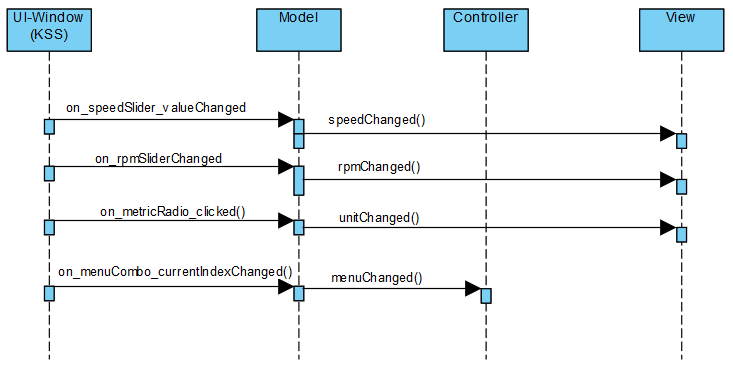
\includegraphics[width=\textwidth]{img/5_implementierung/uml_sequenz}
	\caption{Sequenzdiagramm mit beispielhaften Signalverläufen}
	\label{fig:uml_sequenz}
\end{figure}

\subsection{Implementierung des Controllers}
Für die Umsetzung des Controllers gibt es zwei Möglichkeiten. Der Controller kann als eigene Klasse implementiert werden. Qt bietet dafür ein Zustandsautomaten-Frame"=work an. Für den Controller wird vor allem die QState-Klasse und die verschiedenen Transitions benötigt. Damit könnte der Controller wie im Architektur-Konzept vorgesehen umgesetzt werden. Dadurch sind alle Zustände und Zustandsübergänge zentral an einem Ort. Der Entwicklungsaufwand ist dadurch etwas höher.\\

Im Gegensatz dazu könnten alle Zustände auch dezentral in den einzelnen QML-Dateien angelegt werden. In QML existiert dazu die State Funktion. Diese Funktion ermöglicht es verschieden Zustände zu erstellen. In jedem Zustand kann das Erscheinungsbild der QML-Komponente verändert werden. Der Zustand lässt sich zum einen über Wenn-Bedingung ändern, zum anderen kann der Zustand direkt über die Eigenschaft \textit{state} gewechselt werden. Diese Vorgehensweise erspart die Erstellung einer eigenen Klasse für den Controller, allerdings leidet darunter die Übersichtlichkeit aber einer bestimmten Menge von Zuständen.\\

\subsection{Implementierung der View}
Die View hängt stark vom verwendeten Framework ab. Daher ist im Architektur-Konzept kein UML-Diagramm dafür vorgesehen. Die Implementierung der View mit Qt ist zum größten Teil bereits durch die Umsetzung der Use Cases in den vorherigen Kapiteln abgedeckt. Allerdings wurde die View im Qt Design Studio umgesetzt, die View muss daher noch in das QtCreator Projekt implementiert werden.\\

Um ein Qt Design Studio Projekt in ein QtCreator Projekt zu Konvertieren reicht es der Anleitung in der Dokumentation von Qt zu folgen.\\

Die View ist damit in das QtCreator Projekt eingebunden. Anschließend muss eine Verbindung zum Model hergestellt werden. Zunächst muss QML mitgeteilt werden, dass das Model existiert. Mit der Funktion \textit{setContextProperty()} kann in QML zumindest auf das Model zugegriffen werden. Damit auch ein Zugriff auf die Unterklassen (Speedo, Tacho, etc.) möglich ist, muss mit der Funktion \textit{qRegisterMetaType()} jede Unterklasse registriert werden. Dadurch kann die View auf die Werte im Model zugreifen. Der Geschwindigkeitswert kann dann mit \textit{Model.speedo.speed} ausgelesen werden.\\
% \newpage
% % !TEX root = Hauptdatei.tex
\section{Zusammenfassung und Ausblick}\label{ausblick}
%Zusammenfassung

%Architektur
Das Ziel der Arbeit bestand darin, ein Konzept für Instrument Cluster zu entwickeln und umzusetzen. In Kapitel 3 wurde dazu eine mögliche Softwarearchitektur nach dem \ac{MVC}-Muster erarbeitet. Diese Softwarearchitektur ist nach den Vorgaben des \ac{MVC}-Musters entwickelt worden. Die Architektur soll außerdem die Möglichkeit geben, große Teile der Software immer wieder zu verwenden um den Entwicklungsaufwand zu minimieren.\\

Die View ist im Zusammenhang mit Qt dadurch komplett losgelöst vom Model. Theoretisch muss das Model nur einmal entwickelt werden und kann dann für jedes weitere Projekt benutzt werden. Die View holt sich die Daten, die sie benötigt aus dem Model und stellt alles grafisch dar. Mit ein und dem selben Model können allerdings mehrere verschiedene Views bedient werden, so wie es das \ac{MVC}-Muster vorsieht. Die komplette Logik liegt dabei im Model, lediglich designspezifische Berechnungen werden in der View durchgeführt.\\

%Toolsuche
Ein weiteres Ziel der Arbeit, war es ein geeignetes Tool für die Umsetzung zu finden. Dafür wurden verschiedene Use Cases definiert, um eine Vergleichbarkeit zu schaffen. Insgesamt wurden zwei Tools getestet zum einen Storyboard und zum anderen Qt. Die Use Cases wurden in beiden Frameworks umgesetzt. Der Gewinner dieses Vergleichs war Qt, da alle wichtigen Use Cases umgesetzt werden konnten, im Gegensatz zu Storyboard.\\

%Umsetzung
Die Umsetzung der einzelnen Entwurfsmuster erfolgte in Qt zum einen in C++ oder durch Qt eigene Funktionen. In Tabelle \ref{tab:patterns_model} ist eine Übersicht über die Umsetzung der Entwurfsmuster des Models dargestellt. Für das Model konnten alle im Konzept vorgesehenen Entwurfsmuster verwendet werden.\\

\begin{table}[htb]
	\caption[Umsetzung der Entwurfsmuster (View)]{Umsetzung der Entwurfsmuster (Model)}
	\label{tab:patterns_model}
	\centering
	\small
	\begin{tabular}{|l|c|}
		\hline
		Entwurfsmuster & Umsetzung \\ \hline
		Factory    & reines C++   \\ \hline
		Singleton & reines C++ \\ \hline
		Observer  & Signals \& Slots bzw. Properties  \\ \hline
	\end{tabular}
\end{table}

Der Controller nutzt ebenfalls alle vorher festgelegten Entwurfsmuster. In Tabelle \ref{tab:patterns_controller} ist hierfür eine Übersicht der Entwurfsmuster des Controllers aufgelistet. Das State-Entwurfsmuster z.B. kann durch zwei verschiedene Möglichkeiten umgesetzt werden. Zum einen durch die QState-Klasse von Qt oder durch die State-Funktion im Qt Design Studio.\\

\begin{table}[htb]
	\caption[Umsetzung der Entwurfsmuster (Controller)]{Umsetzung der Entwurfsmuster (Controller)}
	\label{tab:patterns_controller}
	\centering
	\small
	\begin{tabular}{|l|c|}
		\hline
		Entwurfsmuster & Umsetzung \\ \hline
		Factory    & reines C++   \\ \hline
		Singleton & reines C++ \\ \hline
 		Observer  & Signals \& Slots bzw. Properties  \\ \hline
 		State & QState bzw. State-Funktion (Qt Design Studio) \\ \hline
		
	\end{tabular}
\end{table}

Für die View kann keine Übersicht erstellt werden, da alles im Qt Design Studio umgesetzt wurde. Hier werden die Entwurfsmuster nicht sichtbar angewandt. Die Umsetzung passiert intern, daher ist von außen nicht einsehbar welche Entwurfsmuster wie verwendet werden. Allerdings lässt sich erkennen wie das Beobachter-Muster umgesetzt wurde. Durch das Property-System ist es der View möglich, die Daten aus dem Model einzulesen. Dieses Muster ist jedoch das einzige, dass sich beobachten lässt.\\

%Ausblick
Um die Erkenntnisse zu validieren, müsste ein voll umfängliches Projekt mit Qt und der erarbeiteten Architektur umgesetzt werden. Das entwickeln der View könnte dadurch vereinfacht werden, indem verschiedene Module in QML-Dateien umgesetzt und an einem zentralen Ort gespeichert werden. Diese QML-Dateien könnten dadurch immer wieder verwendet werden, nur die Grafiken müssten ausgetauscht werden. Ein Nadelinstrument beispielsweise funktioniert immer ähnlich. Es verändern sich die Grafiken und eventuell der Bereich, in dem sich die Nadel bewegt. Die Nadel bewegt sich immer kreisförmig. Ein Variante der Geschwindigkeitsanzeige wäre ein Balken der sich füllt. Diese Art von Geschwindigkeitsanzeige benötigt eine neue QML-Datei, welche später aber ebenfalls wiederverwendet werden kann. Durch die Zerteilung in einzelne Komponenten ergibt sich die Möglichkeit, die Komponenten die benötigt werden zusammen zu kopieren. Das heißt es könnte einen Assistenten geben, der eine komplette Auswahl an Komponenten bietet, aus der ausgewählt wird, was für das Projekt benötigt wird. Das Projekt kann quasi zusammengeklickt werden. Im Anschluss wird ein QtCreator Projekt vom Assistenten zusammengestellt. \\



  

% \newpage



%\input{7_zusammenfassung_und_ausblick}

%%%%%%% ENDE %%%%%%%%%%%%

%% Beispiel für Bild mit Fußnote
\begin{figure}[htb]
 \centering
 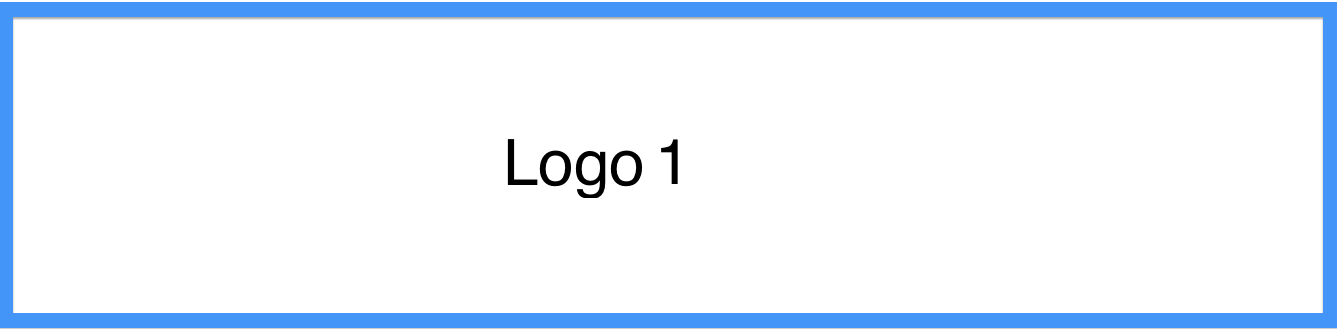
\includegraphics[width=0.4\textwidth,angle=45]{abb/logo1}
 \caption[Beispiel einer Bildbeschreibung]{Beispiel einer Bildbeschreibung\footnotemark}
\label{fig:beispiel1}
\end{figure}
\footnotetext{Bildquelle: Beispiel einer Bildquelle}

% Beispiel für Bildintegration
\begin{figure}[htb]
 \centering
 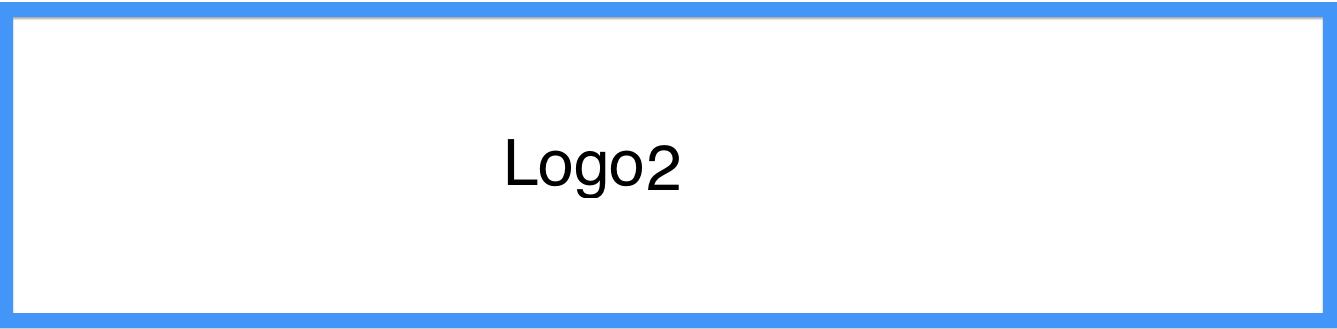
\includegraphics[width=0.3\textwidth,angle=0]{abb/logo2}
 \caption[Beschreibung]{Beschreibung}
\label{fig:Beschreibung}
\end{figure}

% Beispiel: Referenz auf Abbildung
Abbildung~\ref{fig:Beschreibung} [S.\pageref{fig:Beschreibung}]

% Beispiel: Tabelle 
\begin{center}
  \begin{tabular}{ | l | c | }
    \hline
    Überschrift 1 & Überschrift 2 \\ \hline \hline
    Info 1 & Info 2 \\ \hline
    Info 3 & Info 4 \\ \hline
    \hline
    \multicolumn{2}{|c|}{Info in einer Zelle} \\
    \hline
  \end{tabular}
\end{center}


% Beispiel für Quellcode Listings
\lstset{language=xml}
\begin{lstlisting}[frame=htrbl, caption={Die Datei {\normalfont \ttfamily  data-config.xml} dient als Beispiel für XML Quellcode}, label={lst:dataconfigxml}]
<dataConfig>
  <dataSource type="JdbcDataSource" 
              driver="com.mysql.jdbc.Driver"
              url="jdbc:mysql://localhost/bms_db"
              user="root" 
              password=""/>
  <document>
    <entity name="id"
        query="select id, htmlBody, sentDate, sentFrom, subject, textBody
        from mail">
    <field column="id" name="id"/>
    <field column="htmlBody" name="text"/>
    <field column="sentDate" name="sentDate"/>
    <field column="sentFrom" name="sentFrom"/>
    <field column="subject"  name="subject"/>
    <field column="textBody" name="text"/>
    </entity>
  </document>
</dataConfig>
\end{lstlisting}

\lstset{language=java}
\begin{lstlisting}[frame=htrbl, caption={Das Listing zeigt Java Quellcode}, label={lst:result2}]
/* generate TagCloud */
Cloud cloud = new Cloud();
cloud.setMaxWeight(_maxSizeOfText);
cloud.setMinWeight(_minSizeOfText);
cloud.setTagCase(Case.LOWER);
	    
/* evaluate context and find additional stopwords */
String query = getContextQuery(_context);
List<String> contextStoplist = new ArrayList<String>();
contextStoplist = getStopwordsFromDB(query);
	    
/* append context stoplist */
while(contextStoplist != null && !contextStoplist.isEmpty())
  _stoplist.add(contextStoplist.remove(0));
	    
/* add cloud filters */
if (_stoplist != null) {
  DictionaryFilter df = new DictionaryFilter(_stoplist);
  cloud.addInputFilter(df);
}
/* remove empty tags */
NonNullFilter<Tag> nnf = new NonNullFilter<Tag>();
cloud.addInputFilter(nnf);

/* set minimum tag length */
MinLengthFilter mlf = new MinLengthFilter(_minTagLength);
cloud.addInputFilter(mlf);

/* add taglist to tagcloud */
cloud.addText(_taglist);

/* set number of shown tags */	    
cloud.setMaxTagsToDisplay(_tagsToDisplay);
\end{lstlisting}


% Beispiel für Formeln
Die Zuordnung aller möglichen Werte, welche eine Zufallsvariable annehmen kann nennt man \emph{Verteilungsfunktion} von $X$.

\begin{quotation}
Die Funktion F: $\mathbb{R} \rightarrow$ [0,1] mit $F(t) = P (X \le t)$ heißt Verteilungsfunktion von $X$.\footnote{Mustermann, vgl.~\cite{mm2009}~[S.55]}
\end{quotation}

\begin{quotation}
Für eine stetige Zufallsvariable $X: \Omega \rightarrow \mathbb{R}$ heißt eine integrierbare, nichtnegative reelle Funktion $w: \mathbb{R} \rightarrow \mathbb{R}$ mit $F(x) = P(X \le x) = \int_{-\infty}^{x} w(t)dt$ die \emph{Dichte} oder \emph{Wahrscheinlichkeitsdichte} der Zufallsvariablen $X$.\footnote{Mustermann, vgl.~\cite{mf2005}~[S.56]}
\end{quotation}


% einfacher Zeilenabstand
\singlespacing

% Literaturliste soll im Inhaltsverzeichnis auftauchen
\newpage
\addcontentsline{toc}{section}{Literaturverzeichnis}
% Literaturverzeichnis anzeigen
\renewcommand\refname{Literaturverzeichnis}

\bibliographystyle{ieeetr}
\bibliography{Hauptdatei}


% 1,5 facher Zeilenabstand
\onehalfspacing

% evtl. Anhang
% \newpage
%\addcontentsline{toc}{section}{Anhang}
%\fancyhead[L]{Anhang} %Kopfzeile links
%\subsection*{Anhang}\label{anhang}

Der Anhang bestehend aus Bildern und Texten...

% Beispiel für Bildintegration
\begin{figure}[htb]
 \centering
 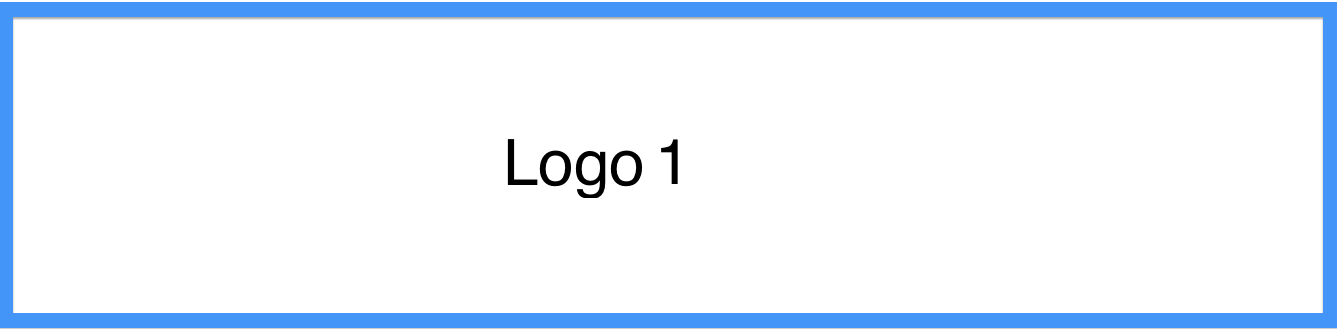
\includegraphics[width=0.3\textwidth,angle=0]{abb/logo1}
 \caption[Abbildung im Anhang]{Abbildung im Anhang}
\label{fig:Abbildung im Anhang}
\end{figure}

Lorem ipsum dolor sit amet, consetetur sadipscing elitr, sed diam nonumy eirmod tempor invidunt ut labore et dolore magna aliquyam erat, sed diam voluptua. At vero eos et accusam et justo duo dolores et ea rebum. Stet clita kasd gubergren, no sea takimata sanctus est Lorem ipsum dolor sit amet. Lorem ipsum dolor sit amet, consetetur sadipscing elitr, sed diam nonumy eirmod tempor invidunt ut labore et dolore magna aliquyam erat, sed diam voluptua. At vero eos et accusam et justo duo dolores et ea rebum. Stet clita kasd gubergren, no sea takimata sanctus est Lorem ipsum dolor sit amet.


% Eidesstattliche Erklärung
% \newpage
% \addcontentsline{toc}{section}{Eidesstattliche Erklärung}
% \section*{Eidesstattliche Erklärung}
\thispagestyle{empty}

\begin{verbatim}

\end{verbatim}

%\begin{LARGE}Eidesstattliche Erklärung\end{LARGE}
%\begin{verbatim}


%\end{verbatim}
Ich versichere, die von mir vorgelegte Arbeit selbstständig verfasst zu haben. Alle Stellen, die wörtlich oder sinngemäß aus veröffentlichten oder nicht veröffentlichten Arbeiten anderer entnommen sind, habe ich als entnommen kenntlich gemacht. Sämtliche Quellen und Hilfsmittel, die ich für die Arbeit benutzt habe, sind angegeben. Die Arbeit hat mit gleichem Inhalt bzw. in wesentlichen Teilen noch keiner anderen Prüfungsbehörde vorgelegen.



\begin{displaymath}
% use packages: array
\begin{array}{ll}
Unterschrift:~~~~~~~~~~~~~~~~~~~~~~~~~~~~~~~~~~~~~~~~~~
& Ort, Datum:~~~~~~~~~~~~~~~~~~~~~~~~~~~~~~~~~~~~~~~~~~
\end{array}
\end{displaymath}

\clearpage


\end{document}
